% Template para Proposta e TCC da EST/UEA -
% Padrão para os cursos do Núcleo de Computação
%
% Elaborado por Elloá B. Guedes
% Adaptado da versão elaborada por:
%                   Jucimar Maia Jr.
%
% Versão 1.3 - 15 de julho de 2022
%
\documentclass[a4paper,titlepage,12pt]{report}


\usepackage[utf8]{inputenc}
\usepackage[OT1]{fontenc}
\usepackage{ae}
\usepackage[brazil]{babel}
\usepackage{a4wide}
\usepackage{comment}
\usepackage[pdftex]{graphicx,color}
\usepackage{graphics}
\usepackage{cite}
\usepackage{longtable}
\usepackage{float}
\usepackage{fancyvrb}
\usepackage{fancyhdr}
\usepackage{setspace}
\usepackage{amsmath}
\usepackage{lscape}
\usepackage{textcase}
\usepackage{anysize}
\usepackage{setspace}
\usepackage{booktabs}
\usepackage{url}
\usepackage{subfig}
\usepackage{cite}
\usepackage[alf]{abntex2cite}
\usepackage{pdfpages}

\marginsize{20mm}{20mm}{20mm}{15mm}


% unidades de medida no SI
\usepackage{siunitx}
\sisetup{output-decimal-marker = {,}, group-minimum-digits=3, group-separator={.},binary-units=true}
\DeclareSIUnit{\pixel}{\text{px}}


%% Cabeçalhos
\renewcommand{\topfraction}{1}
\renewcommand{\bottomfraction}{1}
\renewcommand{\floatpagefraction}{1}
\renewcommand{\textfraction}{0}
%\renewcommand{\baselinestretch}{2}
\doublespacing %espaçamento duplo
\sloppy

%% Nomes
\floatstyle{plain}  %%% tipos: plain, boxed, ruled
\newfloat{codigo}{tbp}{lop}[section]
\floatname{codigo}{Código}

%%% nome para ser usado no sumário

\newcommand{\listofcodename}{Lista de C\'{o}digos}



% RESUMO ----------------------------------------------------------------------------------------------------------------------------------------------------------------------

\newcommand{\resumo}[1]{
\begin{center} \LARGE \bf Resumo \end{center}

\vskip 4em
\input{#1}

\newpage

}

% ABSTRACT ----------------------------------------------------------------------------------------------------------------------------------------------------------------------

\newcommand{\abstractt}[1]{
\begin{center} \LARGE \bf Abstract \end{center}

\vskip 4em
\input{#1}

\newpage

}

% Sumário -----------
\newcommand{\sumario}{
\renewcommand{\contentsname}{Sum\'{a}rio}
\tableofcontents
\addcontentsline{toc}{chapter}{\listtablename}
\listoftables

\newpage
\addcontentsline{toc}{chapter}{\listfigurename}
\listoffigures
% \addcontentsline{toc}{chapter}{\listofcodename}
% \listof{codigo}{\listofcodename}  % Lista de Códigos

\clearpage
}

\pagestyle{plain}

\newcommand{\folhaRosto}[5]{

\thispagestyle{empty}
\begin{center}
\textbf{\\[0.4em]\MakeUppercase{#2} \\[5cm]}
\textbf{\MakeUppercase{#1}\\[96pt]}

\end{center}

\hspace*{8cm}
\begin{minipage}{8cm}
Trabalho de Conclus\~{a}o de Curso
apresentado \`{a} banca avaliadora do Curso de Engenharia de Computa\c{c}\~{a}o, da
Escola Superior de Tecnologia, da Universidade do Estado do Amazonas, como
pr\'e-requisito para obten\c{c}\~{a}o do t\'{\i}tulo de Engenheiro de Computa\c{c}\~{a}o.\\[40pt]
\end{minipage}

\begin{center}
Orientador(a): #3 \\[12ex]
Manaus -- #4 -- #5\\
\end{center}


\pagenumbering{roman}
\newpage
}




%% Preencha aqui os seguintes dados
\def \titulo{Uma Aplicação de Redes Neurais Convolucionais\\ Regionais para Detecção de Malária}
\def \orientador{Prof. Dra. Elloá Barreto Guedes da Costa}
\def \nome{Jesus Dourado de Albuquerque}
\def \mes{Março}
\def \ano{2023}

\begin{document}

\folhaRosto{\titulo}{\nome}{\orientador}{\mes}{\ano}

% Edite os seguintes arquivos para alterar as informações necessárias
% \begin{center} \LARGE \bf Ficha Catalográfica \end{center}


\begin{enumerate}
    \item Estas instruções \textbf{não} devem ser entregues aos avaliadores do trabalho nas ocasiões dos TCCs 1 e 2. Portanto, comente a linha que importa este arquivo;
    \item A ficha catalográfica deve ser elaborada após a defesa do TCC2, quando você concluir as correções sugeridas pela banca e validar a versão final com o/a professor(a) orientador(a);
    \item Acessar \url{http://repositorioinstitucional.uea.edu.br:8080/ficha/ficha_catalografica.php} e preencher as informações requeridas para elaborar a ficha catalográfica;
    \item Incluir o pdf gerado na subpasta \emph{source} com o nome \texttt{ficha.pdf};
    \item Apagar todo o conteúdo deste arquivo e deixar apenas o comando a seguir:
    \begin{verbatim}
        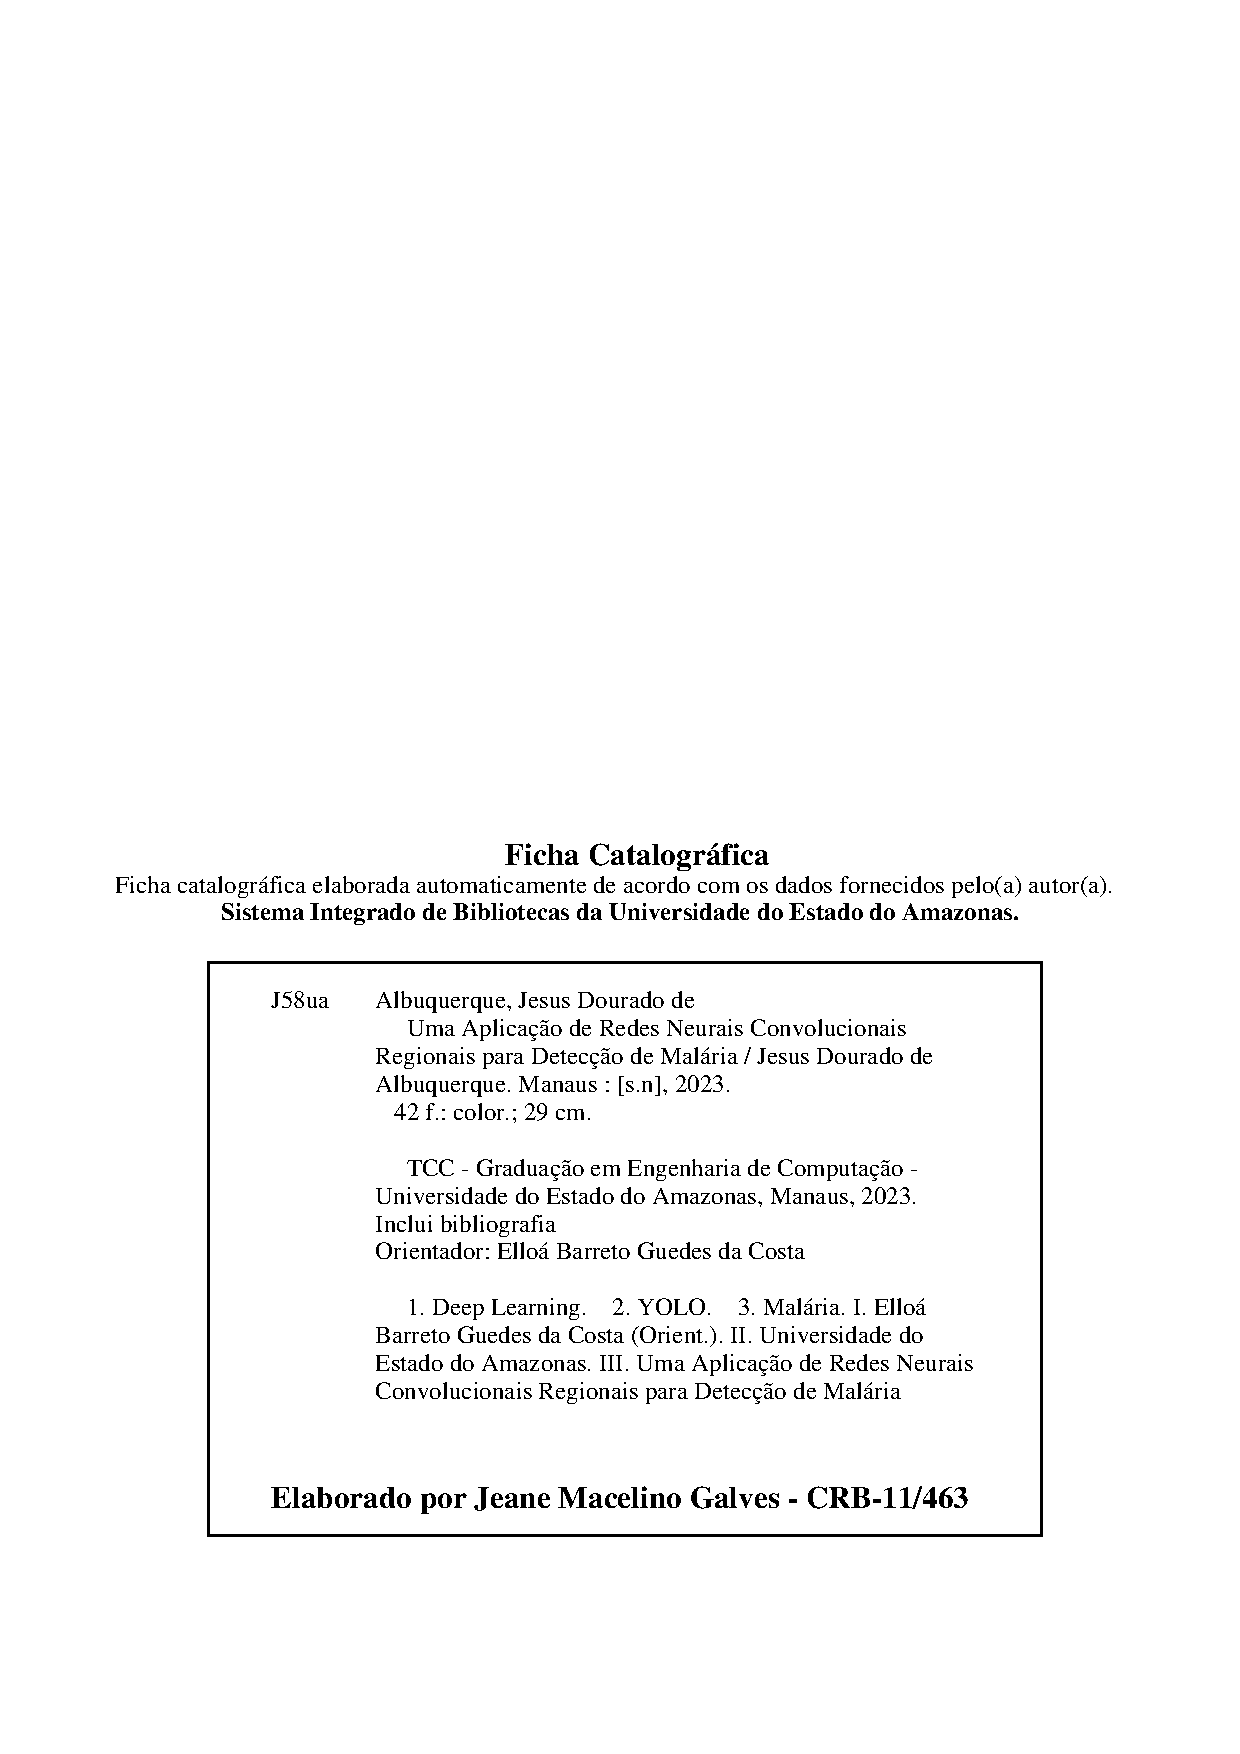
\includepdf[pages=-]{./source/ficha.pdf}
    \end{verbatim}
\end{enumerate}

\newpage

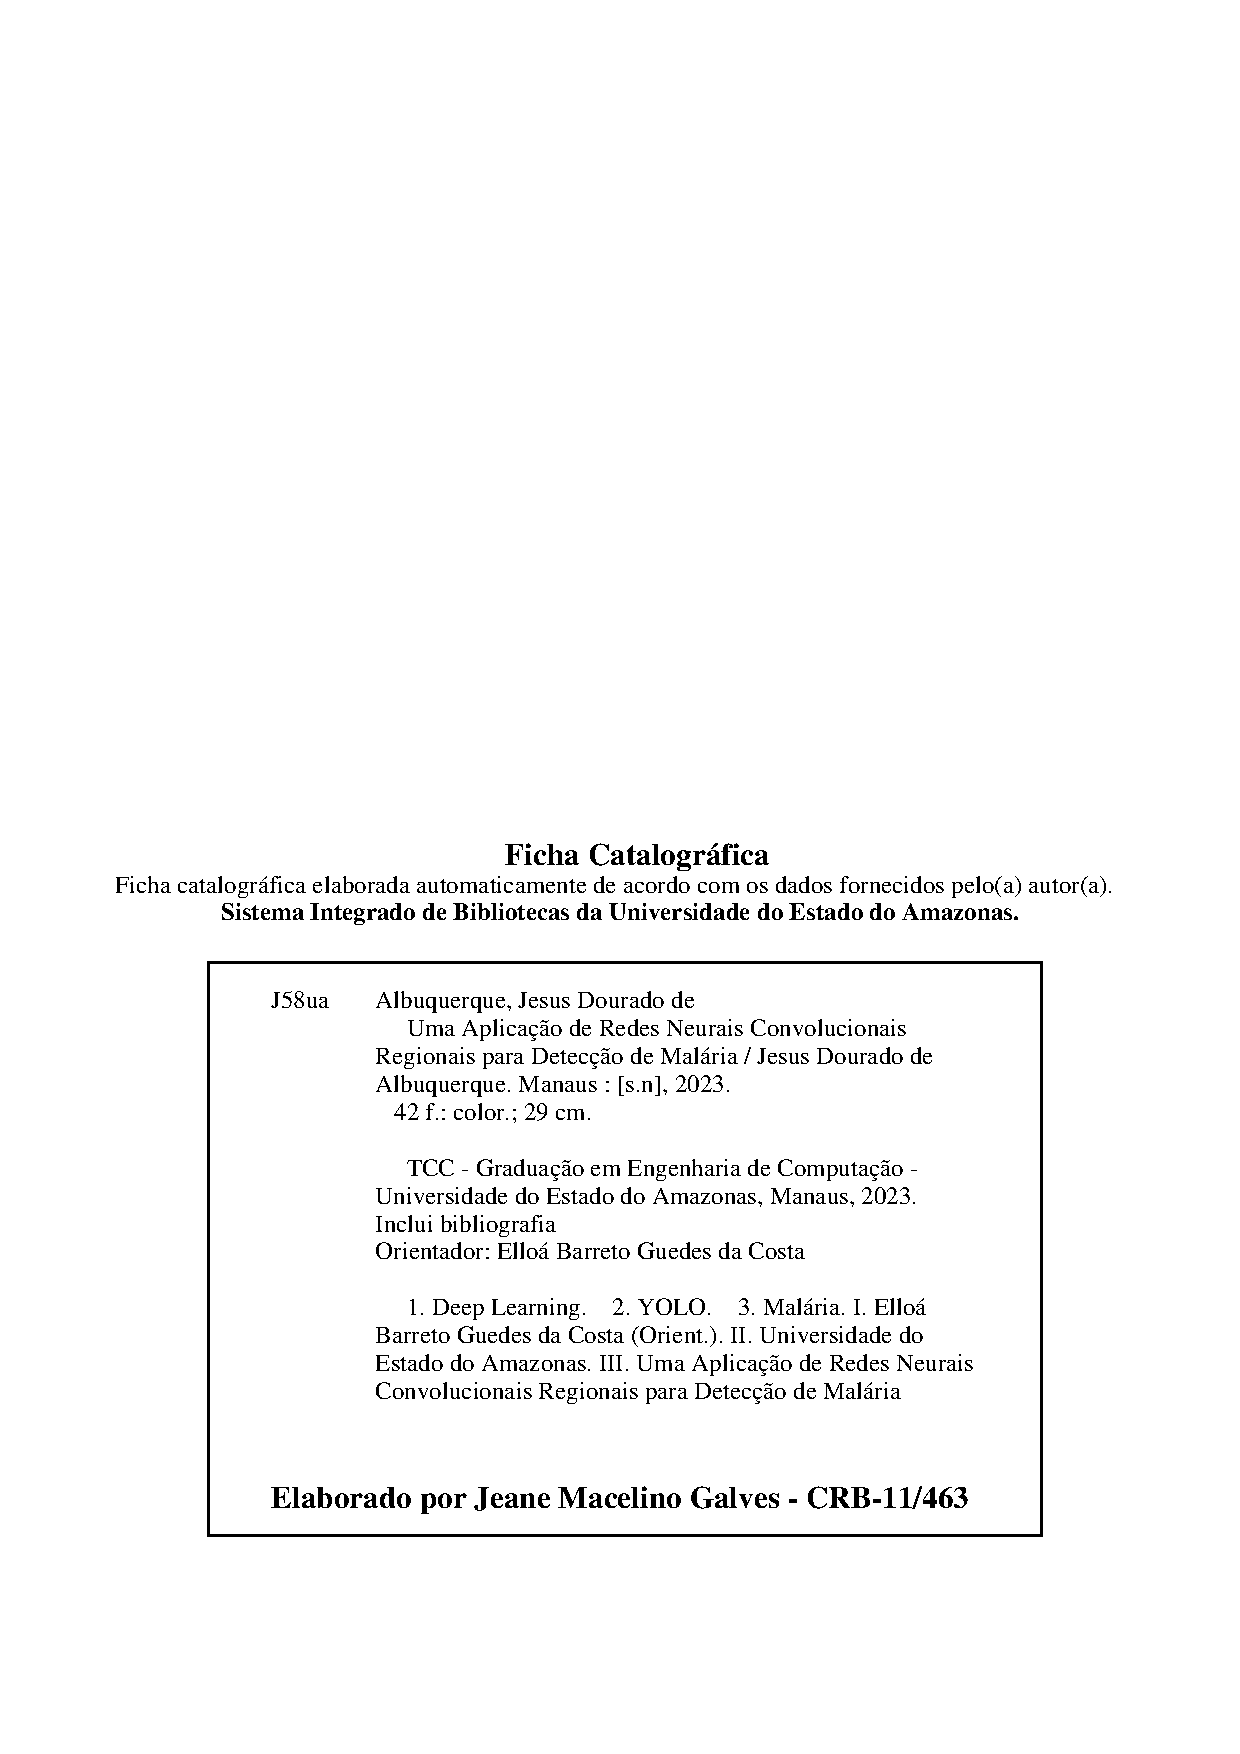
\includepdf[pages=-]{./source/ficha.pdf}
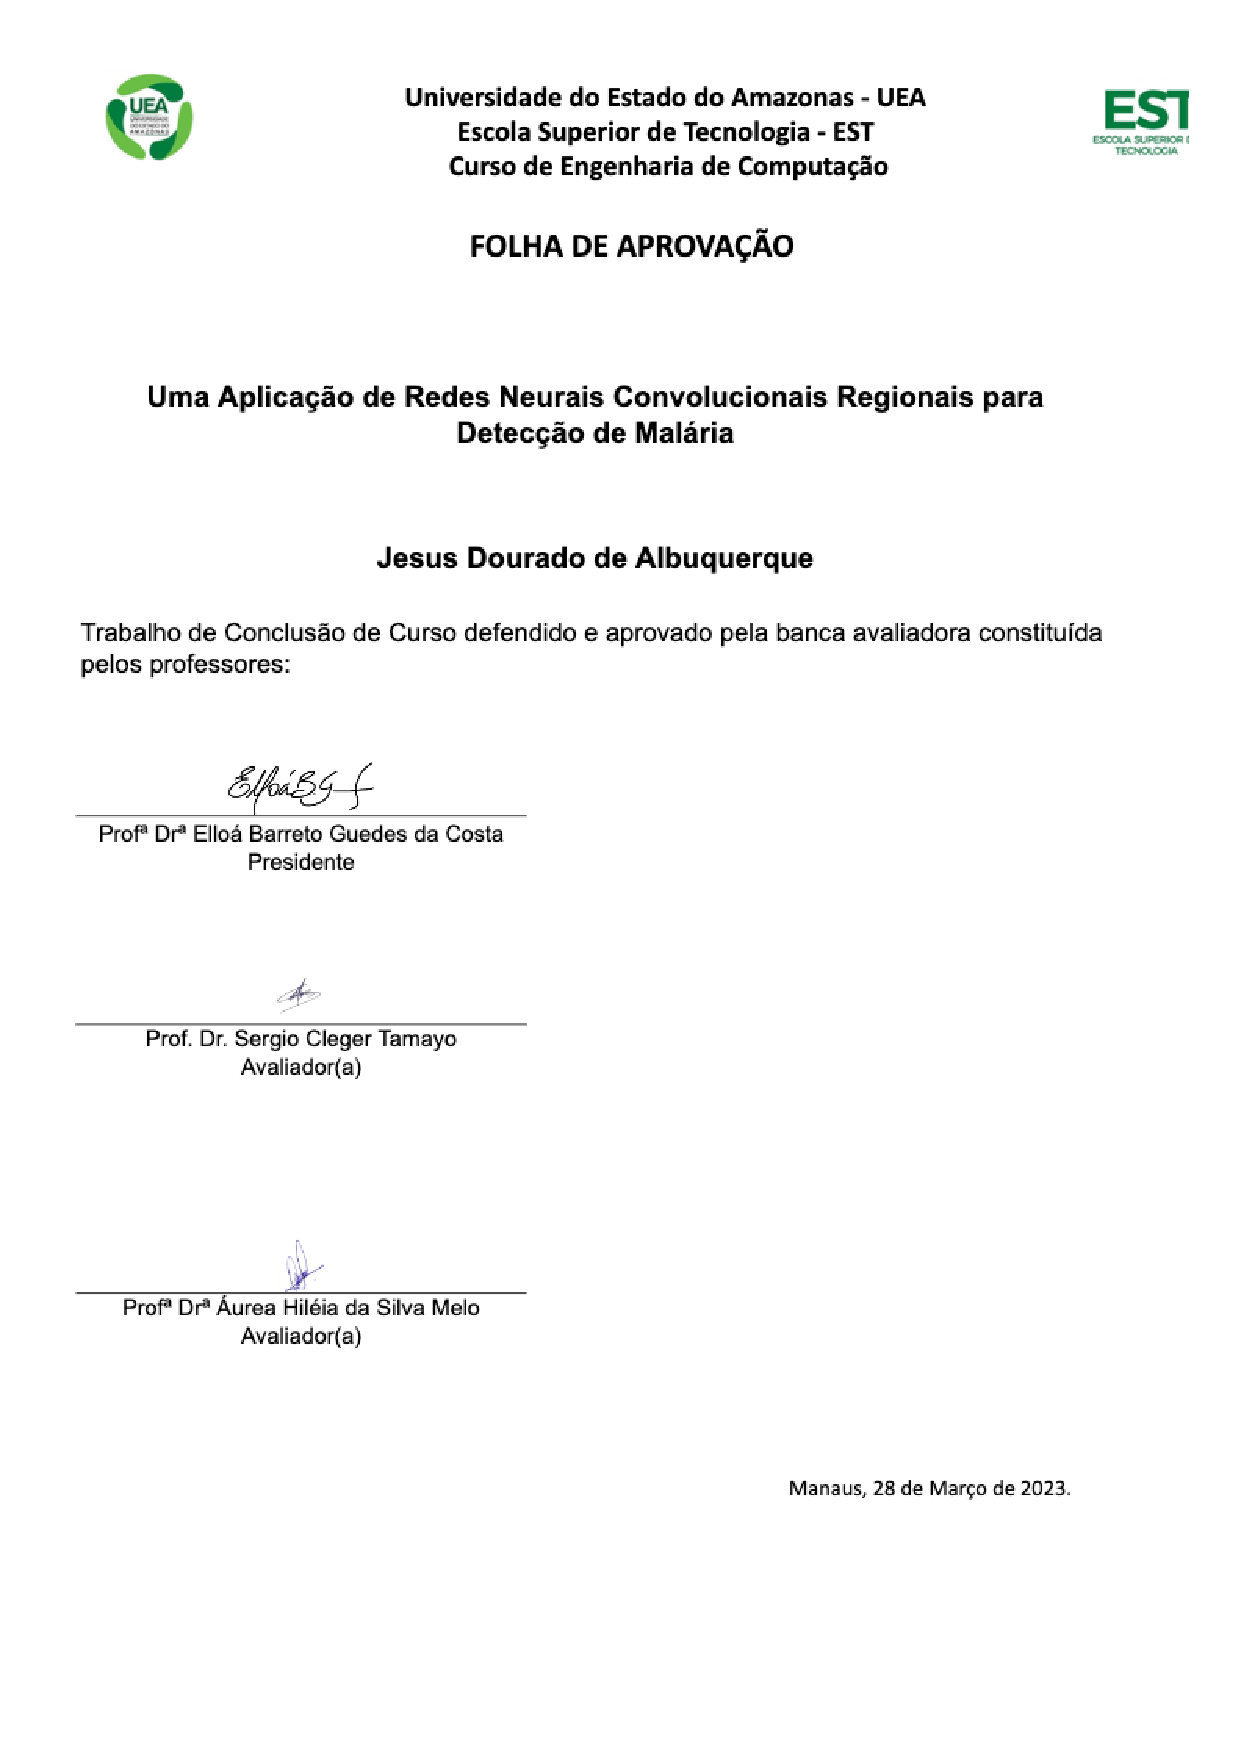
\includepdf[pages=-]{./source/assinaturas.pdf}


% Indique onde esta o arquivo do resumo
\resumo{./files/RESUMO.tex}
% Idem para o abstract
\abstractt{./files/ABSTRACT.tex}


\sumario

% Configuração de cabeçalhos
\pagestyle{fancy}
\renewcommand{\chaptermark}[1]{\markboth{#1}{}}
\renewcommand{\sectionmark}[1]{\markright{#1}}
\renewcommand{\headrulewidth}{0.5pt}
\newcommand{\rom}{\fontfamily{cmr}\fontseries{m}\fontsize{10}{12}\selectfont}
\fancyhf{} \fancyhead[LE,RO]{\rom\thepage}
\fancyhead[LO]{\rom\rightmark} \fancyhead[RE]{\rom\leftmark}
\fancypagestyle{plain}{
    \fancyhead{} % get rid of headers
    \renewcommand{\headrulewidth}{0pt} % and the line
 }


\pagenumbering{arabic}



% Seus capítulos vão aqui --------
% \chapter{Exemplo}

\section{Tabela com o Pacote Booktabs}

Um exemplo de tabela com o pacote booktabs pode ser visto na Tabela \ref{tabela:exemplo}. A explicação das tabelas sempre vem em cima e esse padrão deve ser respeitado. A numeração é automática e a inserção no índice também. Legal né? \cite{Bennett:QuantumInformationSurvey}

Basta quebrar uma linha para criar um novo parágrafo. Neste parágrafo vou contar que tabelas no \LaTeX dão um pouco de trabalho, mas nada que com paciência não se resolva. Veja os links com dicas que coloquei nos comentários do arquivo \texttt{index.tex}.

\begin{table}[ht!]
\caption{Esta é uma tabela básica em \LaTeX com o pacote booktabs.} \label{tabela:exemplo}
\center{
\begin{tabular}{cccc}
\toprule
Parte 1 & Parte 2 & Parte 3 & Parte 4\\
\midrule
0,415 & 1,365 & 1,98 & 2,05\\
1,36  & 45,5  & 7,98 & 3,01\\
2,36  & 1,35  & 0,15 & 5,32\\
\bottomrule
\end{tabular}}
\end{table}



\section{Inserção de Figuras}

Você pode inserir figuras JPG no \LaTeX! Veja o caso da Figura \ref{fig:exemplo}. Se você quiser outras configurações e dicas, veja o seguinte endereço: \url{http://en.wikibooks.org/wiki/LaTeX/Floats,_Figures_and_Captions}.

A explicação da figura sempre vem embaixo da mesma. Isto aqui é um novo parágrafo apenas para ilustrar a idéia geral de como escrever.

\begin{figure}[H]
\centering
\caption{Um exemplo de figura JPG inserida no \LaTeX.} \label{fig:exemplo}
\includegraphics[width=0.4\textwidth]{./img/exemplo.jpg}\\
\small{Elaborado pelo autor.}
\end{figure}

Pode inserir várias figuras lado a lado também. Um exemplo está reproduzido a seguir.

\begin{figure}[H]
  \centering
  \caption{Canal clássico cuja obtenção da capacidade erro-zero é não-trivial.}
  \subfloat[\ ]{\label{fig:exG5}\includegraphics[width=0.3\textwidth]{./img/001}}
  \hspace{0.5cm}
  \subfloat[\ ]{\label{fig:exG52}\includegraphics[width=0.3\textwidth]{./img/002}}
  \hspace{0.5cm}
  \subfloat[\ ]{\label{fig:exG53}\includegraphics[width=0.3\textwidth]{./img/003}}\\
  \small{Elaborado por Bacon}
\end{figure}

\section{Referências Bibliográficas no Padrão ABNT}

Para gerar versões corretas do \textsc{Bib}\TeX das suas referências, recomenda-se usar o DOI no caso de artigos e o ISBN no caso de livros. Em posse dessas informações, consulte os seguintes links:

\begin{enumerate}
    \item \url{https://www.bibtex.com/c/doi-to-bibtex-converter/}
    \item \url{https://www.bibtex.com/c/isbn-to-bibtex-converter/}
    \item \url{http://doi-to-bibtex-converter.herokuapp.com/}
    \item \url{https://www.doi2bib.org/}
\end{enumerate}

Para saber mais sobre os tipos de referências \textsc{Bib}\TeX e seus significados, consultar a documentação oficial em \url{https://www.bibtex.com/e/entry-types/}.

Este template está integrado com o pacote \texttt{abnt2cite} que produz as referências no padrão ABNT NBR 6023.

\chapter{Introdução}

A malária é uma doença causada pelo protozoário do gênero \emph{Plasmodium} e transmitida pela fêmea do mosquito do gênero \emph{Anopheles}. No Brasil, existem três espécies do \emph{Plasmodium} que transmitem malária para seres humanos: \emph{P.\@ vivax}, \emph{P.\@ malariae} e \emph{P.\@ falciparum}, sendo esta última considerada a mais grave por causar alterações estruturais nos glóbulos vermelhos \cite{Gomes:2011,Loiola:2002}.

Quanto à enfermidade, de acordo com a Fundação Oswaldo Cruz (FIOCRUZ), trata-se de uma doença infecciosa.  Em um paciente portador do protozoário, o seu estado clínico é variável a partir do início da infecção, mas listam-se os seguintes sintomas como os mais comuns: febre alta e intermitente, dores musculares, cefaleia e delírios. Quando o tratamento é negligenciado, a doença pode se agravar e manifestar sintomas mais severos, tais como desorientação, convulsões, vômitos, sonolência ou excitação e, eventualmente, levar o paciente a óbito \cite{FIOCRUZ:Site}.

A malária ainda é considerada um problema grave de saúde no mundo, sendo uma das principais doenças letais em regiões tropicais e subtropicais ao redor do globo. De acordo com o Relatório Mundial de Malária de 2019 produzido pela Organização Mundial de Saúde (OMS), foram registrados 228 milhões de casos e 405 mil mortes em âmbito global, em que a grande maioria ocorreu na África \cite{OMS:Malaria2019}.

No Brasil, a malária é uma doença de notificação compulsória e, portanto, todos os casos suspeitos ou confirmados devem ser, obrigatoriamente, notificados às autoridades de saúde \cite{Brasil:DecretoMalaria}. A série histórica dos casos de malária no Brasil foi iniciada em 1959 e até o o ano de 2005 possuía forte tendência crescente, vindo a diminuir significativamente até o ano de 2013 \cite{Boletim:2013}. Entre os anos de 2017 a 2019 há uma queda percentual de $\SI{19,3}{\percent}$ no número de casos, mas há suspeita de subnotificação levantada pelas autoridades de saúde \cite{Boletim:Malaria2020}. Mais recentemente, os anos de 2020 e 2021 registraram 141 mil e 135 mil casos, respectivamente \cite{Boletim:Malaria2022}. Ressalta-se que, em todo o período observado, a maioria dos casos da doença ocorreu na região Amazônica (Acre, Amapá, Amazonas, Maranhão, Mato Grosso, Pará, Rondônia, Roraima e Tocantins), área endêmica para a doença \cite{Brasil:SINAN}.

O diagnóstico da malária é feito atualmente por meio da análise microscópica de lâminas contendo amostra de sangue coletadas pelo método da gota espessa ou ainda por testes rápidos de diagnóstico (RDTs, do inglês \emph{Rapid diagnostic tests}) \cite{OMS:Malaria2019}. Segundo um estudo recente, os RDTs possuem uma variação de desempenho de detecção da doença a depender da localização geográfica considerada e da idade do paciente, o que ressalta sua limitação. Apesar disso, os autores recomendam-os para uso em áreas remotas e reforçam a análise microscópica como técnica de referência para o diagnóstico \cite{Berzosa:MalariaDiagnostico}. A análise de amostras sanguíneas para detecção de malária requer não apenas equipamentos de boa qualidade, mas também habilidade em microscopia, o que é dificultada pela má disposição de treinamento para os profissionais da área, o que enseja diagnósticos incorretos \cite{Paz:Habilidade}.

Uma estratégia para contornar as dificuldades enfrentadas para o diagnóstico da malária é considerar o papel relevante das soluções computacionais baseadas em métodos e técnicas de \emph{Deep Learning} para problemas de Visão Computacional na área de Saúde, tais como em Imagiologia Médica e  Microscopia \cite{Shen:SurveyMedico,Lee:SurveyMedico,Xing:SurveyMedico}. Essa sub-área emergente da Inteligência Artificial baseia-se principalmente no uso de Redes Neurais Convolucionais Profundas (CNNs, do inglês \emph{Convolutional Neural Networks} para extração sucessiva de características hierárquicas em dados de alta dimensionalidade \cite{Goodfellow:Livro}, permitindo aplicações de classificação, detecção e segmentação em imagens mediante Aprendizado Supervisado a partir de conjuntos massivos de dados \cite{Chollet:2017,Khan:2018}.

É intuitivo, assim, conjecturar acerca do potencial de aplicação de métodos de \emph{Deep Learning} em imagens microscópicas para colaborar no diagnóstico de malária. Esta questão já foi explorada em outros trabalhos da literatura, os quais consideraram a tarefa de classificação binária quanto à presença ou ausência do protozoário em uma dada célula sanguínea, previamente segmentada manualmente ou conforme algum método de Visão Computacional tradicional \cite{Felipe:2022,Yang:2020}. Embora os resultados obtidos por estes autores denotem bom desempenho das CNNs nesta tarefa, dependem crucialmente de uma etapa de pré-processamento para isolamento das múltiplas células contidas em uma imagem microscópica.

Considerando as limitações observadas na literatura, este trabalho de conclusão visou investigar a viabilidade no uso de métodos de \emph{Deep Learning} para detecção de protozoários causadores de malária em uma dada imagem microscópica fornecida como entrada. A vantagem de uma solução desta natureza é a delimitação e localização de cada parasita na imagem, permitindo a posterior supervisão por um especialista humano; favorecendo a contagem dos protozoários, o que é crucial para determinar a estratégia de tratamento; e colaborando para mitigar os erros de diagnóstico em face das habilidades requeridas pelos microscopistas humanos nesta tarefa.

\section{Objetivos}

O objetivo geral deste trabalho consistiu em avaliar modelos de \emph{Deep Learning} para detecção de malária em imagens microscópicas. Para alcançar este objetivo, foi necessário contemplar as seguintes metas:

\begin{enumerate}
    \item Identificar e preparar uma base de dados da literatura no domínio da detecção de malária;
    \item Elaborar e conduzir um estudo de caso experimental para treinamento e avaliação comparativa das arquiteturas de CNNs para detecção de objetos;
    \item Avaliar e analisar os resultados obtidos de maneira qualitativa e quantitativa.
\end{enumerate}

\section{Justificativa}

Mesmo tendo sido descoberta no final do Século XIX, a malária ainda é uma doença endêmica em todo o mundo, com um grande quantitativo de casos e óbitos, em que a principal justificativa para a perda de vidas é o diagnóstico tardio combinado com a falta de acesso aos recursos para tratamento \cite{OMS:Malaria2019}. No Brasil, embora o tratamento seja gratuito,  mais de $\SI{70}{\percent}$ dos casos ocorreram em áreas rurais ou regiões indígenas \cite{Boletim:Malaria2022}, o que se mostra um desafio em um país de dimensões continentais. Em todo o caso, o diagnóstico de referência da malária é feito via análise microscópica, o que depende de profissionais altamente especializados \cite{Paz:Habilidade}.

Colaborar para o desenvolvimento de métodos automáticos e inteligentes para o diagnóstico de malária pode mitigar o fardo dessa doença, antecipando o diagnóstico e, consequentemente, o tratamento. Isto pode ser especialmente crucial para as populações mais vulneráveis e aquelas que residem em regiões remotas, em que não há disponibilidade de serviços de saúde e tampouco infraestrutura de alta qualidade para microscopia. Ademais, é possível também ampliar a quantidade de testes realizados, permitindo um melhor monitoramento de populações residentes em áreas endêmicas. Ressalta-se, entretanto, que no escopo deste trabalho de conclusão de curso não haverá coleta de dados diretamente com sujeitos e que tampouco os modelos propostos e avaliados  serão utilizados ou testados em cenários reais. Se viáveis, estes passos podem ocorrer em momentos posteriores no contexto da proposição de outros projetos de pesquisa e com a devida supervisão de Comitê de Ética.

Por fim, deve-se mencionar a importância da realização deste trabalho com vistas a colaborar com as atividades desenvolvidas pelo LSI, uma iniciativa do Grupo de Pesquisas em Sistemas Inteligentes da Escola Superior de Tecnologia (EST) da UEA.

\section{Metodologia}

A metodologia utilizada para o desenvolvimento das atividades presentes neste trabalho, com o intuito de atingir os objetivos especificados, é descrita a seguir:

\begin{enumerate}
    \item Estudo dos conceitos relativos às CNNs perante tarefas de detecção (R-CNNs);
    \item Levantamento do ferramental tecnológico para implementação das R-CNNs;
    \item Identificação e análise exploratória de uma base de dados disponível na literatura voltada para a tarefa de Visão Computacional de detecção de malária;
    \item Identificação de arquiteturas de R-CNNs do estado da arte para problemas de detecção, especialmente da Família YOLO;
    \item Conceber um cenário experimental para avaliação dos modelos de R-CNNs para detecção de malária;
    \item Treinamento dos modelos;
    \item Aferição das métricas de desempenho no teste dos modelos;
    \item Escrita da proposta de Trabalho de Conclusão de Curso;
    \item Defesa da proposta de Trabalho de Conclusão de Curso;
    \item Escrita do Trabalho de Conclusão de Curso;
    \item Defesa do Trabalho de Conclusão de Curso.
 \end{enumerate}

\section{Organização do Documento}

Este documento está organizado como segue: os fundamentos teóricos que embasam o trabalho, incluindo conceitos de \emph{Deep Learning} com CNNs e sua aplicação na detecção de objetos encontram-se dispostos no Capítulo \ref{cap:fundamentacao}, incluindo também uma apresentação de contribuições relacionadas ao problema já existentes na literatura. Os materiais e métodos adotados para a solução proposta encontram-se discriminados no Capítulo \ref{cap:metodologia}. Os resultados obtidos são apresentados e discutidos no Capítulo \ref{cap:resultados}. Por fim, as considerações finais podem ser consultadas no Capítulo \ref{cap:considera}.
\chapter{Fundamentação Teórica} \label{cap:fundamentacao}

Nas seções a seguir encontra-se uma breve apresentação dos conceitos que fundamentaram a realização deste trabalho. Uma visão geral sobre \emph{Deep Learning} com CNNs encontra-se disponível na Seção \ref{sec:deepLearning}; a aplicação de CNNs na tarefa de detecção de objetos é detalhada na Seção \ref{sec:fundamenta:deteccao}; as características das arquiteturas das R-CNNs da Família YOLO são apresentadas na Seção \ref{sec:fund:yolo}; por fim, os trabalhos correlatos da literatura são apresentados e discutidos na Seção \ref{sec:fund:relacionados}.

\section{\emph{Deep Learning} com CNNs} \label{sec:deepLearning}
%!TEX root=../../sbc-template.tex
%% Ideia global da seção
% O que é Deep Learning?
% Quais as características das Redes Neurais Convolucionais?

O Aprendizado de Máquina (AM) é uma sub-área da Inteligência Artificial que lida com algoritmos que são melhorados de forma implícita a partir de exemplos do domínio considerado \cite{Faceli:Livro}. A maioria dos problemas abordados com modelos, métodos e técnicas dessa área compreendem tarefas complexas cuja solução analítica por meio dos algoritmos tradicionais é inviável ou até mesmo impraticável \cite{Brink:MachineLearningLivro}.

No contexto de AM, ``aprender'' é um termo que denota o processo de busca automática pela melhor representação da informação que viabiliza a transformação dos dados de entrada com o intuito de facilitar a resolução de uma dada tarefa considerada, a exemplo de uma classificação binária \cite{Chollet:2017}. Para efetuar essa busca automática, entretanto, faz-se necessária a intervenção humana altamente especializada para escolha dos melhores modelos, parâmetros e hiper-parâmetros, os quais são diretamente relacionados ao sucesso na resolução da tarefa considerada \cite{Khan:2018}.

Com o intuito de tornar o processo de aprendizado mais independente, \emph{Deep Learning} (DL), uma sub-área de AM, têm se destacado em diversos contextos práticos, pois objetiva aprender automaticamente, por meio de diversas camadas hierárquicas e sucessivas, múltiplas representações complexas de dados de entrada multimodais (imagens, sons, vídeo, etc.), aumentado assim o domínio de problemas que podem ser abordados \cite{Buduma:2018}. Para o domínio de DL, as CNNs são o modelo de referência para múltiplas tarefas. As mesmas são um tipo recente de Rede Neural Artificial \emph{Feedforward Multilayer Perceptron} (RNA MLP), as quais compõem o paradigma conexionista da Inteligência Artificial \cite{Russel:IABiblia}. As RNAs MLP são compostas por um conjunto de unidades básicas de processamento, denominadas neurônios artificiais, que são fortemente interconectados e organizados segundo camadas, operando nos dados de entrada com o objetivo de inferir uma função que aprenda as respectivas saídas, conforme o paradigma de Aprendizado Supervisionado \cite{Khan:2018}.

Os neurônios artificiais são inspirados nos neurônios biológicos e funcionam de forma independente como unidades computacionais simples que recebem sinais de entrada e atribui-lhes pesos, produzindo um sinal de saída usando uma função de ativação. A Figura \ref{fig:neuronio} ilustra a estrutura de um neurônio abstrato com $n$ entradas, em que cada canal de entrada é um valor $x_i \in \mathbbm{R}$. Cada entrada possui um peso associado $w_i \in \mathbbm{R}$, e o corpo do neurônio calcula a soma ponderada das entradas e sujeita esse valor a uma função de ativação $f(\cdot)$, que define o limite no qual o neurônio produz um sinal de saída ativado \cite{Teresa:Livro}.

\begin{figure}[ht]
\centering
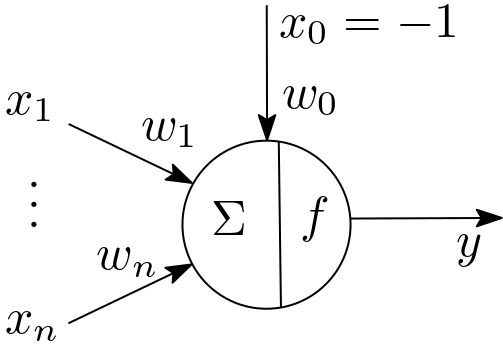
\includegraphics[width=.5\textwidth]{./img/neuronio.png}
\caption{Modelo abstrato de um neurônio artificial. Fonte: \cite{Teresa:Livro}.}
\label{fig:neuronio}
\end{figure}

O poder computacional de um neurônio individual é limitado às funções linearmente separáveis. Ao dispor os neurônios em camadas e conectá-los a todos os neurônios da camada seguinte, conforme estabelecido nas RNAs MLP, torna-se possível uma transformação sucessiva nos dados de entrada que os tornam linearmente separáveis à medida que se aproximam da camada de saída \cite{Faceli:Livro}, conforme ilustrado na Figura \ref{fig:mlp}.

\begin{figure}[ht]
\centering
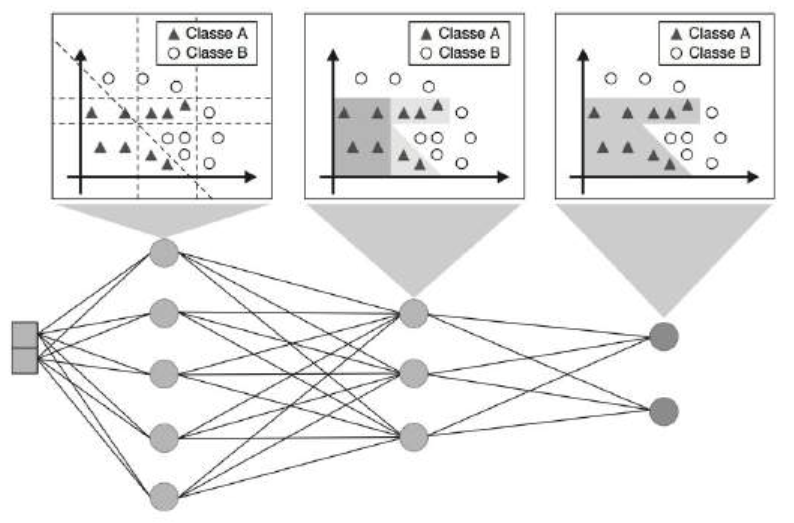
\includegraphics[width=.8\textwidth]{./img/mlp.png}
\caption{Papel desempenhado pelos neurônios em cada camada de uma RNA MLP. Fonte: \cite{Faceli:Livro}.}
\label{fig:mlp}
\end{figure}

O aprendizado das RNAs se dá por meio de um processo iterativo de ajustes aplicado a seus pesos, fazendo com que o modelo obtenha melhor desempenho, normalmente medido pela acurácia preditiva. Esses algoritmos, são formados por um conjunto de regras bem definidas que determinam quando e como dever ser alterado o valor de cada peso \cite{Faceli:Livro}. Um método popular para o aprendizado supervisionado de MLPs é o algoritmo de \emph{backpropagation}, que consiste em duas fases: uma fase pra frente (\emph{forward}) e outra pra trás (\emph{backwards}). Na fase \emph{forward}, os pesos sinápticos da rede são fixos e o sinal de entrada é propagado pela rede, camada por camada, até atingir a saída. Na segunda fase \emph{backwards}, um sinal de erro é produzido comparando a saída da rede com uma resposta desejada. O sinal de erro resultante é propagado através da rede, camada por camada, porém a propagação é realizada pra trás \cite{Faceli:Livro,Haykin:NeuralNetworksBook}. Nesta segunda fase, ajustes sucessivos são feitos nos pesos da rede utilizando o algoritmo do gradiente descendente \cite{Teresa:Livro}.

As CNNs são uma categoria de RNAs especialmente voltadas para lidar com dados de alta dimensionalidade, tais como imagens, áudio, vídeo, etc. Elas operam de maneira muito semelhante às RNAs MLP, mas com uma diferenças fundamentais no tocante aos neurônios e aos tipos de camada. Os neurônios artificiais convolucionais são caracterizados por um filtro que é convoluído com a entrada, permitindo uma extração apropriada de características frente ao tipo de dado de entrada, pois são capazes de abstrair características como texturas, contornos, cores, etc. As camadas compostas de neurônios convolucionais são chamadas de camadas convolucionais \cite{Khan:2018}.

As CNNs também fazem uso de camadas de \emph{pooling}, tipicamente dispostas após as camadas convolucionais, com vistas a promover uma redução de dimensionalidade, produzindo representações condensadas das entradas. As diversas camadas convolucionais e de \emph{pooling} na arquitetura de uma CNN são responsáveis pela extração automática de características da entrada, as quais passam por camadas densas, tipicamente dispostas ao final da CNN, com vistas a produzir a saída desejada para a tarefa em questão (classificação, regressão, etc.) \cite{Buduma:2018,Chollet:2017}.

Como a extração de características nas CNNs é automática e massiva, é importante utilizar alguma estratégia para descartar valores que podem estar associados à ruído ou que possuem pouca influência na saída do modelo. Isso é feito com camadas de \emph{Dropout}, as quais são compostas de neurônios com limiar para descartar aleatoriamente certas conexões ao longo do treino, colaborando para a regularização e para a diminuição no número de parâmetros ajustáveis das CNNs \cite{Buduma:2018,Chollet:2017}.

As CNNs são tipicamente utilizadas perante o paradigma de Aprendizado Supervisionado com especial destaque para tarefas de classificação em Visão Computacional, representando o estado da arte em diversos problemas nesse domínio \cite{Khan:2018}. Citam-se algumas arquiteturas canônicas de CNNs, tais como, LeNet, AlexNet, Inception e VGG-16, as quais obtiveram desempenho notável em diversas edições do \emph{ImageNet Large Scale Visual Recognition Challenge} (LSVRC) \cite{ILSVRC15}.


\section{Detecção de Objetos com Redes Neurais Convolucionais} \label{sec:fundamenta:deteccao}
%!TEX root=../../sbc-template.tex

A detecção e o reconhecimento de objetos são componentes chave para a maioria dos sistemas de visão computacional e determinam o desempenho de muitos aplicativos, como rastreamento, recuperação, vigilância por vídeo e legendagem de imagens. O desempenho da detecção e reconhecimento de objetos depende muito da qualidade das características extraídas e da robustez dos modelos, uma vez que a aparência das imagens pode ser influenciada por diversos fatores, como condições de iluminação, pose, refletância dos objetos e características intrínsecas das câmeras \cite{Jiang:2019}. Por isso que, nos últimos anos, as redes neurais profundas ganharam espaço nos problemas mais complexos da atualidade como processamento de imagens e visão computacional. A Figura \ref{fig:example-detection} ilustra a detecção de várias classes para uma mesma entrada.

\begin{figure}[H]
    \centering
    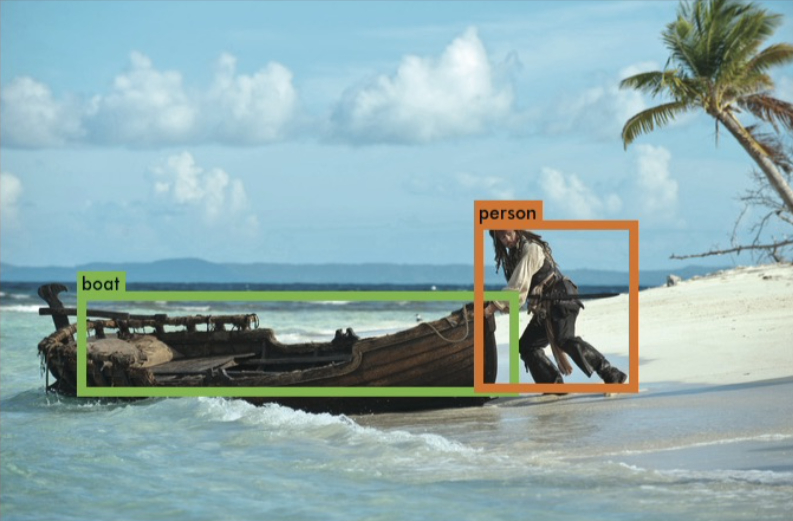
\includegraphics[width=.7\textwidth]{img/example-detection.png}
    \caption{Tarefa de detecção de objetos sendo realizada. Fonte: \cite{Yolo:2015}}
    \label{fig:example-detection}
\end{figure}

É importante salientar que a classificação de uma imagem, isto é, um modelo classificar o conteúdo de uma foto, por exemplo, é diferente de detectar exatamente em que área da foto o objeto encontra-se. Com isso, é possível perceber que os modelos que abordam essa tarefas precisam ser mais robustos pois existe agora uma nova etapa na qual o modelo precisa realizar: definir na imagem quais os limites da entidade em questão. Em resumo, o modelo, para detecção de objetos numa imagem, deve ser capaz de identificar a localização de uma ou mais entidades (as classes) além de emitir qual classe ela(s) pertence(m) \cite{Michelucci:2019}.

A métrica necessária para verificar a qualidade dessa tarefa é justamente a interseção da área correspondente ao objeto (resultado esperado) em relação à área detectada sobre a união dessas áreas em questão, conhecida também como Interseção sobre União (IoU) \cite{Chollet:2017}. O desafio está em detectar as áreas das entidades na imagem. Uma das primeiras estratégias que solucionaram esse problema é a Aproximação da Janela Deslizante: uma certa área (a janela deslizante) igual ou menor que a imagem total é inicialmente definida e percorre todas as combinações possíveis com a imagem original, calculando o IoU. Em seguida, outra janela deslizante é definida com outro tamanho e o processo é refeito. No fim, verifica-se qual IoU foi o mais satisfatório para o resultado final da detecção da entidade. Essa estratégia é bastante custosa pois podem existir milhares de combinações possíveis em cada teste, razão pela qual não é muito utilizada \cite{Michelucci:2019}.

Outra estratégia para a detecção é conhecida como Region-Based CNN (R-CNN), ou CNN Baseada em Regiões. Como a estratégia das janelas deslizantes necessita de muitas combinações, a baseada em regiões propõe inicialmente 2000 regiões na imagem. Em seguida as regiões adjacentes são unidas baseadas em características similares como cor, textura e forma, sendo possível visualizar a técnica na Figura \ref{fig:selective-search}. Então, com menos regiões para serem analisadas, o cálculo de IoU é também realizado e a melhor métrica acaba escolhendo também a melhor região para o resultado \cite{Michelucci:2019}.

\begin{figure}[H]
    \centering
    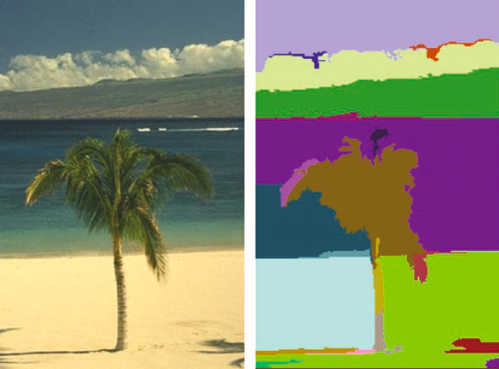
\includegraphics[width=.7\textwidth]{img/selective-search.png}
    \caption{Pesquisa seletiva destacando regiões de interesse. Fonte: \cite{Michelucci:2019}}
    \label{fig:selective-search}
\end{figure}

Como as R-CNN são modelos mais complexos devido ao janelamento, uma solução para torná-las mais rápidas foi desenvolvida: a chamada Fast R-CNN. A razão pela qual esse algoritmo é mais rápido que o R-CNN está no fato de que torna-se desnecessário alimentar 2000 propostas de região para a rede neural convolucional, o processo é realizado uma única vez com a extração de mapa de características da imagem, similar às características semelhantes das regiões inicializadas nas R-CNN \cite{Michelucci:2019}.

Mesmo as Fast R-CNN tendo se mostrado mais rápidas que as R-CNN convencionais, o custo para treinar o modelo ainda é alto visto que a pesquisa para selecionar as regiões propostas é ainda gargalo do algoritmo. Com isso, uma outra solução para essa etapa foi desenvolvida: utilizar uma outra rede neural para aprender as regiões de dados rotulados, removendo então a etapa demorada de procura seletiva das regiões. Assim, esse modelo foi chamado de Faster R-CNN por ser significativamente mais rápido que R-CNN e Fast R-CNN \cite{Michelucci:2019}.



\section{Família YOLO} \label{sec:fund:yolo}
%!TEX root=../../sbc-template.tex

Com a popularização das R-CNNs e o crescente interesse prático nas tarefas de detecção de objetos, em 2016 foi proposta a R-CNN YOLO (acrônimo para \emph{You Only Look Once}), a qual se propõe a realizar as tarefas de localização e classificação de múltiplos objetos em uma única etapa (\emph{single-shot}) \cite{Redmon:YOLOoriginal}. Essa R-CNN mostrou-se significativamente mais rápida para detecção do que os modelos anteriores do mesmo tipo disponíveis na literatura \cite{Michelucci:2019}.

Conforme ilustrado na Fig. \ref{fig:yolo_grid}, a abordagem de detecção de objetos por R-CNNs YOLO consiste nos seguintes passos: primeiramente há a divisão da imagem de entrada em uma grade de dimensões $S \times S$; em seguida, para cada célula, há uma verificação se há um objeto cujo centro é englobado pela mesma; para as células em que tal verificação foi afirmativa, calcula-se a quantidade $B$ de caixas delimitadores com seus respectivos coeficientes de confiança -- obtidos por meio da multiplicação da métrica IoU (do inglês, \emph{Intersection Over Union}) com a probabilidade da célula conter um certo objeto de uma dada classe -- refletindo numericamente o quão acurada está uma caixa delimitadora que contém o objeto; por fim, células adjacentes com alta confiança para um mesmo tipo de objeto são unificadas, culminando na previsão das coordenadas das caixas e seus respectivos rótulos \cite{Michelucci:2019}.

\begin{figure}[H]
    \centering
    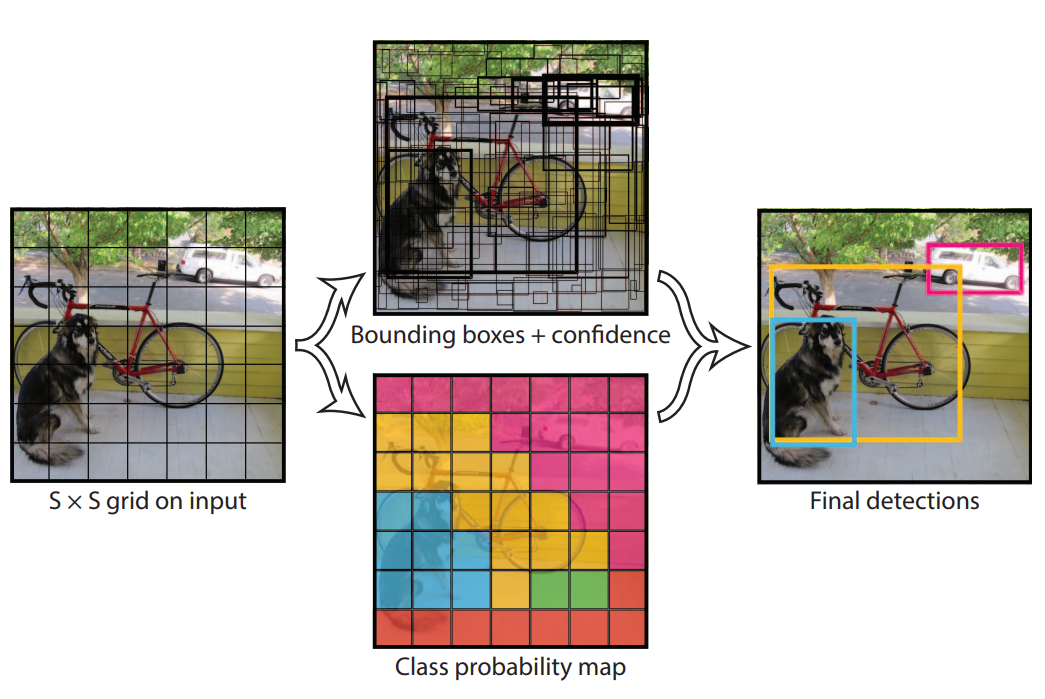
\includegraphics[width=0.70\textwidth]{img/yolo-approach}
    \caption{Abordagem da YOLO para detecção de objetos.
    Fonte: \cite{Redmon:YOLOoriginal}.}
    \label{fig:yolo_grid}
\end{figure}

A arquitetura utilizada na YOLOv1 (primeira versão) foi inspirada na CNN Inception pré-treinada com pesos oriundos da base de dados ImageNet \cite{ImageNet}. Esta arquitetura é constituída por $20$ camadas convolucionais seguidas por $2$ camadas totalmente conectadas. Ao invés de usar os módulos Inception originais, os autores da YOLO optaram por utilizar camadas de \emph{pooling} com filtros de dimensões $1\times 1$ para redução de dimensionalidade seguidos de camadas convolucionais com filtros $3 \times 3$, conforme ilustrado na Figura \ref{fig:yolo_arch}.

\begin{figure}[H]
    \centering
    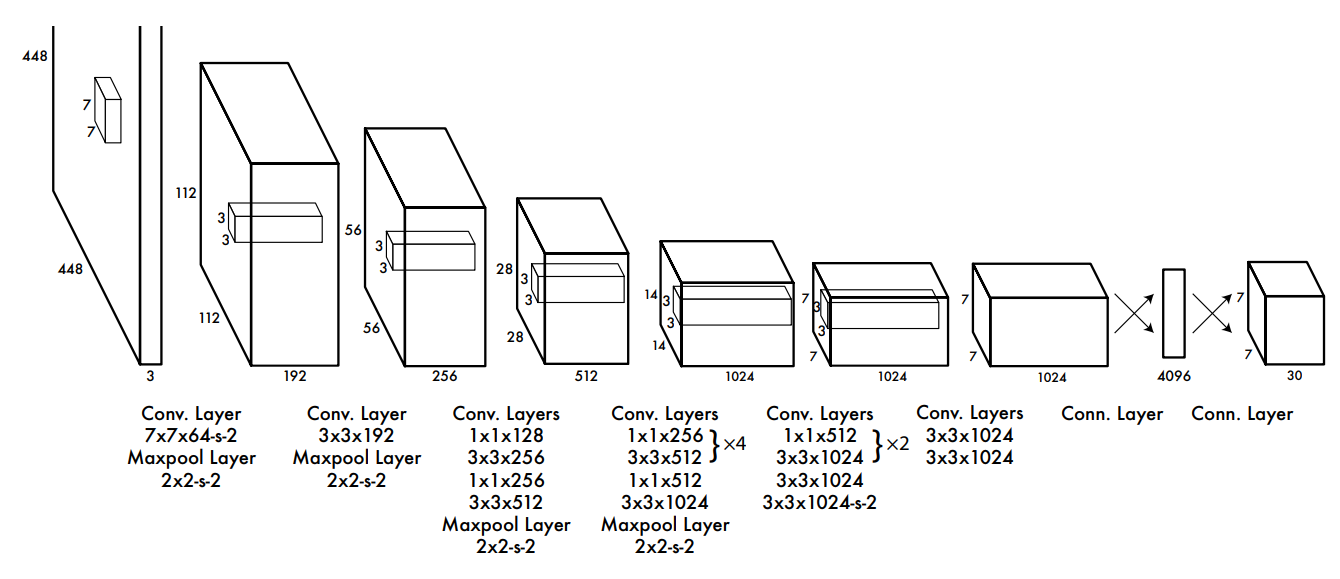
\includegraphics[width=\textwidth]{img/yolo-arquitetura}
    \caption{Arquitetura da CNN utilizada na primeira versão da YOLO.\\ Fonte: \cite{Redmon:YOLOoriginal}.}
    \label{fig:yolo_arch}
\end{figure}

% Seguir para Yolov4,  v5, v6 e v7.

Ao longos dos anos, novas técnicas e melhorias foram incorporadas em versões atualizadas de modelos da Família YOLO. Para a YOLOv4, por exemplo, utilizou-se o \emph{backbone} CSPDarkNet53, tornando-a duas vezes mais rápida que outras arquiteturas de referência na época do seu lançamento. Ainda, comparando com a sua versão anterior (YOLOv3) as métrica AP e FPS foram melhoradas em $\SI{10}{\percent}$ e $\SI{12}{\percent}$, respectivamente \cite{Bochkovski:YOLOv4}.

A YOLOv5 decorreu logo após a proposição da YOLOv4 tendo como maior diferença a implementação do \emph{framework} DarkNet de forma nativa com o Pytorch, o que facilitou drasticamente o treinamento e o \emph{deployment} desse modelo. A principal inovação da YOLOv5 em relação às suas antecessoras foi a introdução do \emph{Mosaic Augmentation}, uma técnica de regularização por meio do aumento artificial de dados que combina quatro imagens em quatro blocos de proporção aleatória. Conforme argumentam seus proponentes, a principal vantagem dessa inovação é a melhoria de desempenho na detecção de objetos pequenos. No sétimo \emph{release}, diferentes versões da YOLOv5 foram propostas para atender domínios específicos, citadas a seguir por ordem crescente de parâmetros e robustez: \emph{Nano}, \emph{Small}, \emph{Medium}, \emph{Large} e \emph{XLarge}. Os modelos mais simples visam aplicações embarcadas por serem mais leves, enquanto os mais complexos foram projetados para problemas mais difíceis, com imagens de maior dimensão, grande número de classes e tamanho de caixas delimitadoras bastante variados \cite{Jocher:YOLOv5}. A Figura \ref{fig:yolov5} ilustra o desempenho das diferentes versões da YOLOv5 perante a base de dados MS COCO \cite{Microsoft:COCO}, um \emph{benchmark} da literatura para detecção de objetos.

\begin{figure}[h!]
    \centering
    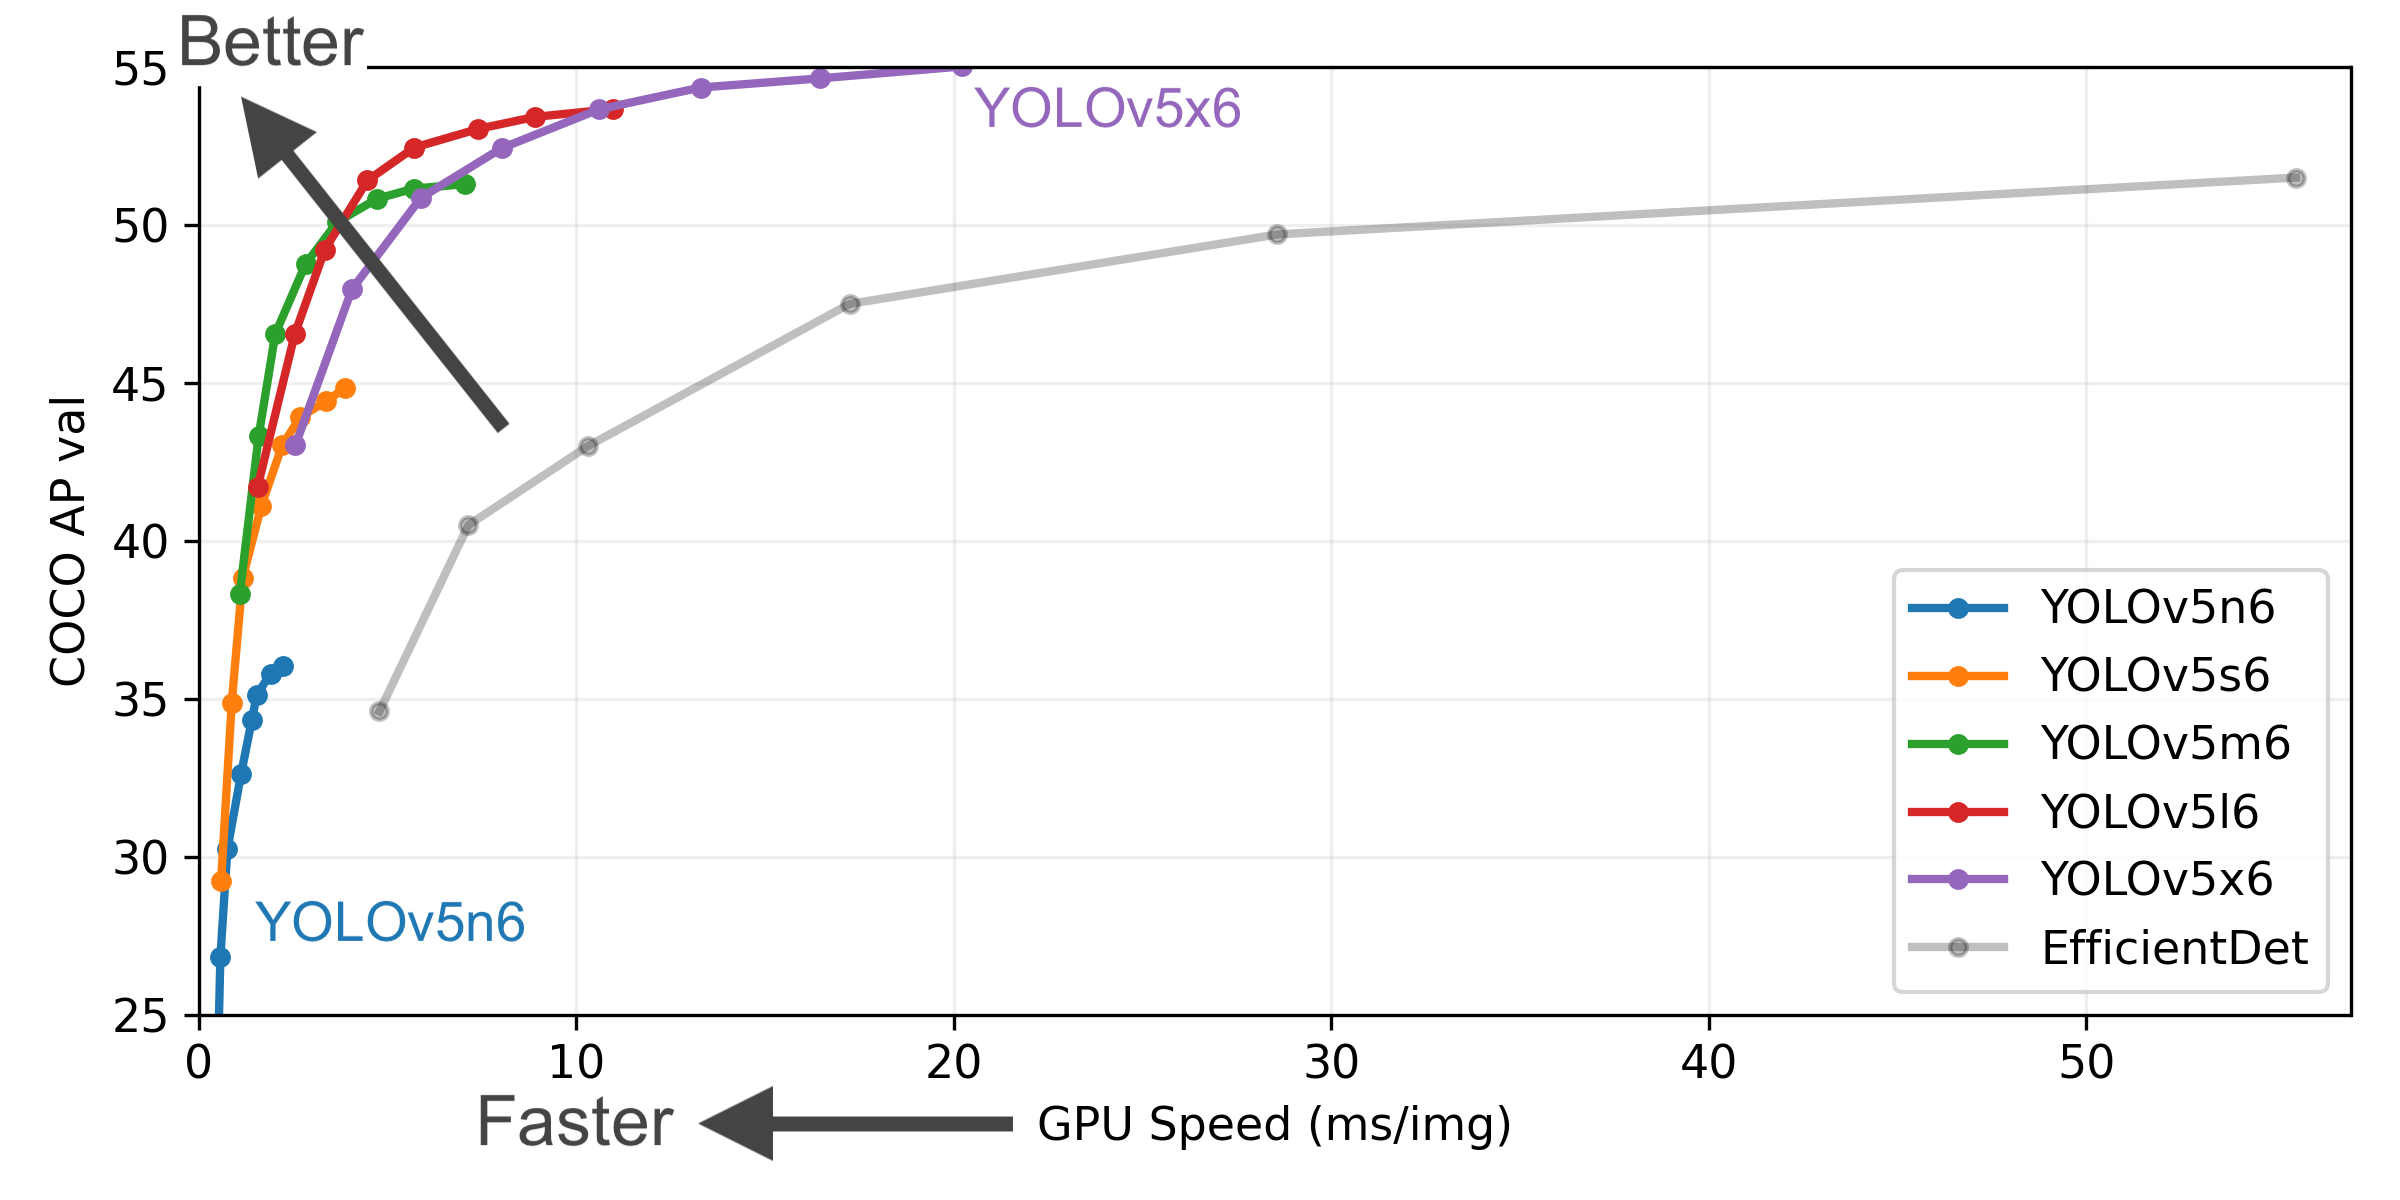
\includegraphics[width=0.8\textwidth]{./img/yolov5}
    \caption{Desempenho dos modelos YOLOv5 perante o MS COCO.\\ Fonte: \cite{Jocher:YOLOv5}.}
    \label{fig:yolov5}
\end{figure}

Outras versões da YOLO foram propostas por diferentes autores, mas nem todas se consolidaram perante a comunidade técnico-científica pois, apesar de apresentarem um bom desempenho no \emph{benchmark} MS COCO, não reproduziam tal eficiência em problemas de outros domínios. Ademais, era notável a dificuldade no treinamento em face da carência de documentação e de uma comunidade pequena de usuários. Como exemplo, cita-se o caso da YOLOv6 \cite{YOLOv6}.


A YOLOv7 deu continuidade ao aprimoramento dos modelos da Família YOLO ao incorporar um processo denominado reparametrização, com o intuito de diminuir o tamanho do modelo para \emph{deployment}, o que é especialmente útil para sistemas embarcados. Também faz uso de \emph{Feature Pyramid Networks} em sua arquitetura, as quais empilham camadas convolucionais e produzem previsões em diferentes escalas, colaborando para um melhor desempenho. Diferentemente das versões anteriores, propôs uma arquitetura padrão e uma estratégia de dimensionamento em escala para outras quantidades de parâmetros, sejam elas maiores ou menores \cite{yolov7}. A Figura \ref{fig:yolo-arch} apresenta uma análise comparativa entre os diferentes modelos da Família YOLO recém propostos na literatura perante o MS COCO.


\begin{figure}[h!]
    \centering
    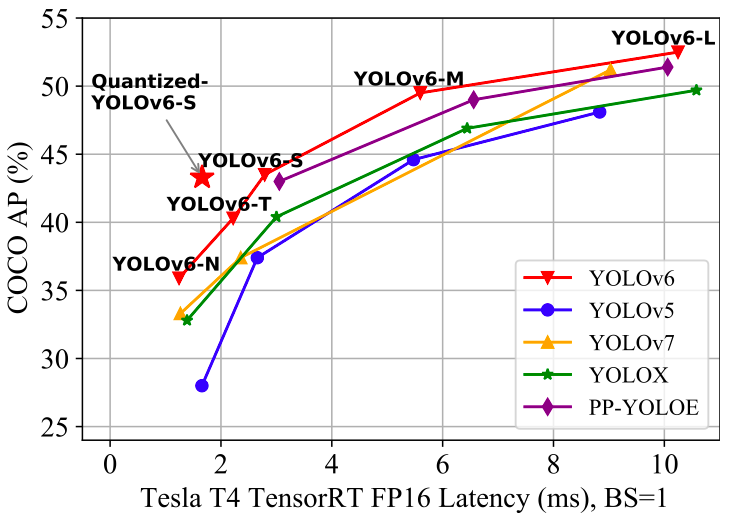
\includegraphics[width=0.75\textwidth]{img/yolo-latest-version}
    \caption{Comparação entre as últimas versões da YOLO propostas na literatura. O eixo vertical denota a eficiência do modelo e o eixo horizontal denota o tempo de treinamento.\\ Fonte: \cite{YOLOv6}.}
    \label{fig:yolo-arch}
\end{figure}

\section{Trabalhos Relacionados} \label{sec:fund:relacionados}
\iffalse \begin{frame}{Trabalhos relacionados}
    \begin{itemize}
        \item Primeiros trabalhos: uso de sensores, tais como acelerômetro e giroscópio, para reconhecer danos por meio da amplitude da vibração detectada \cite{caodl}
        \ \ \newline
        \item \alert{\emph{Global Road Damage Detection Challenge}} (GRDDC):
        \begin{itemize}
            \item \alert{RDD2020}: \emph{Road Damage Detection and Classification dataset} \cite{RDD2020:Dataset2}
            \item Equipes realizaram a etapa de testes em duas bases de dados privadas
            \item $\SI{67}{\percent}$ das melhores soluções utilizaram modelos de família YOLO e as 3 melhores soluções utilizaram comitês de R-CNNs \cite{arya2020global}
            \item \alert{Melhor solução}: $F_1\textrm{-\emph{Score}} \approx 0,67$, YOLOv5, Test Time Augmentation, $3,08$ FPS \cite{Hegde2020:Campeao}
        \end{itemize}
    \end{itemize}
\end{frame}
\fi
%!TEX root=../sbc-template.tex
\chapter{Materiais e Métodos} \label{cap:metodologia}

Este trabalho aborda o problema de Visão Computacional de detecção de protozoários causadores de malária em imagens de lâminas de sangue capturadas por microscópio. Para tanto, considera a tarefa de detecção de objetos de uma única classe perante o paradigma de Aprendizado Supervisionado utilizando R-CNNs da Família YOLO. Para elaborar a solução proposta, os dados experimentais utilizados para aquisição de experiência são apresentados na Seção \ref{sec:metodologia:dados}; o detalhamento dos modelos YOLO, suas versões e parametrizações são apresentados na Seção \ref{sec:metodologia:modelos}; e, por fim, a apresentação da estratégia de validação experimental e da coleta de métricas de desempenho encontram-se na Seção \ref{sec:metodologia:desempenho}.

\section{Dados Experimentais} \label{sec:metodologia:dados}
%!TEX root=../../sbc-template.tex

Os dados experimentais utilizados no escopo desse trabalho são oriundos de uma base de dados pública do Hospital Universitário Chittagong em Bangladesh com $150$ pacientes e $1830$ imagens de lâminas de sangue \cite{Yang:2020}, capturadas por uma câmera de celular conectada a um microscópio. As imagens obtidas possuem a resolução de $\SI[parse-numbers=false]{4032 \times 3024}{\pixel}$ e, para cada uma, existe um arquivo com os rótulos contendo informações dos tamanhos circulares e localizações dos protozoários da malária ou das células brancas do sangue. As anotações relativas às células brancas foram descartadas por não serem do escopo de interesse do problema em questão. No total, havia $\num{84509}$ rótulos para a classe de interesse nos exemplos da base de dados.

Como os modelos da Família YOLO utilizam caixas retangulares para detecção dos objetos, foi necessário realizar uma etapa de pré-processamento para substituir os círculos originalmente disponíveis. Para tanto, calculou-se o raio do círculo e obteve-se entãoo a caixa delimitadora de formato quadrado circunscrita ao círculo, conforme exemplificado na Figura \ref{fig:example-class}.  Ademais, observou-se que $\SI{0.55}{\percent}$ das imagens não possuíam rótulos.

 \begin{figure}[h!]
 	\centering
 	\hfill \subfloat[Imagem sem rótulos]{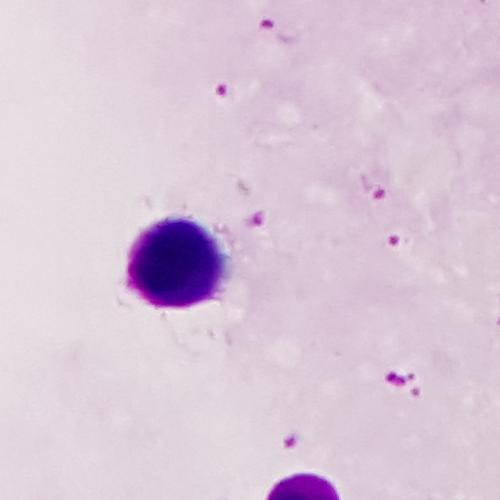
\includegraphics[width=0.32\linewidth]{img/sample/blood-raw.jpg}}
 	\hfill \subfloat[Centroides]{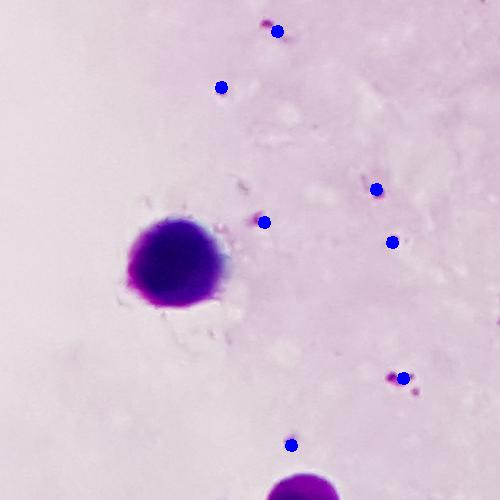
\includegraphics[width=0.32\linewidth]{img/sample/blood-centers.jpg}}
 	\hfill \subfloat[Centroides e caixa delimitadora]{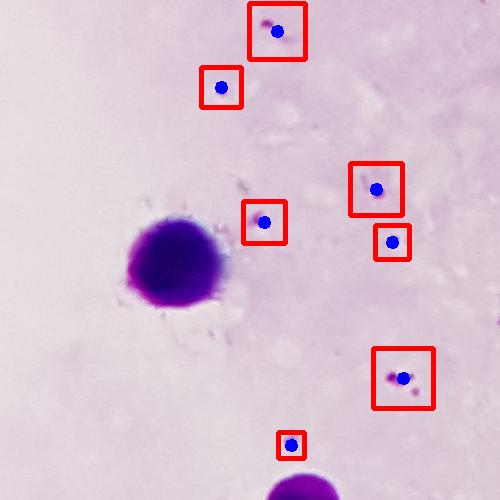
\includegraphics[width=0.32\linewidth]{img/sample/blood-squares.jpg}}
 	\caption{Exemplo com a imagem original, acrescida de centroides e das caixas delimitadoras quadradas.}
 	\label{fig:example-class}
\end{figure}

Ao efetuar uma análise exploratória das imagens e dos rótulos disponíveis nas mesmas, conforme histograma da Figura \ref{fig:histogram}, foi possível perceber que a maioria das imagens ($967$) possuía até $25$ caixas delimitadoras. Do total de imagens,  somente $17$ não possuíam nenhum rótulo ($\SI{0.55}{\percent}$ dos exemplos da base de dados), indicando pacientes saudáveis. Embora não sejam relevantes para o aprendizado de padrões a respeito dos protozoários, colaboram no aprendizado do \emph{background} pelos modelos de detecção com \emph{Deep Learning}. Observou-se também que poucas imagens possuíam mais de $200$ protozoários com caixas delimitadoras, correspondendo a $\SI{2.1}{\percent}$ dos exemplos da base de dados.

 \begin{figure}[ht]
    \centering
    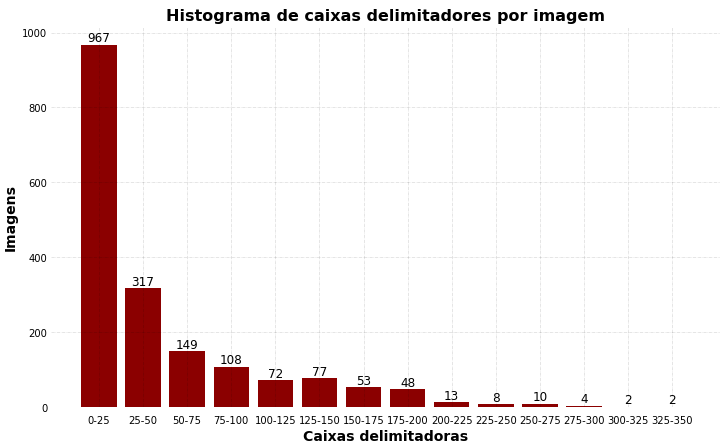
\includegraphics[width=0.9\textwidth]{img/histogram.png}\hfill
    \caption{Histograma da quantidade de caixas delimitadoras por imagens da base de dados.}
    \label{fig:histogram}
\end{figure}

Um mapa de calor foi elaborado para ilustrar a disposição espacial dos rótulos das caixas delimitadoras nas imagens da base de dados, conforme mostrado na Figura \ref{fig:heat-map}. Nota-se uma distribuição uniforme de tais caixas sobre toda a região visível pelo microscópio, o que reforça a dificuldade na tarefa de detecção por não haver boas regiões candidatas na distribuição \emph{a priori} dos exemplos.

\begin{figure}[H]
    \centering
    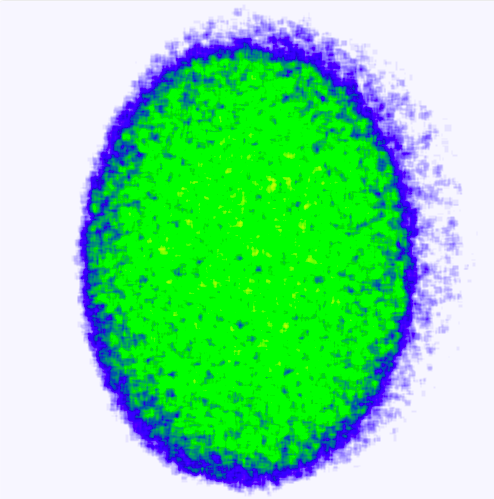
\includegraphics[width=0.7\textwidth,height=0.525\textwidth]{img/heat-map.png}\hfill
    \caption{Mapa de calor da disposição das caixas delimitadoras nos exemplos.}
    \label{fig:heat-map}
\end{figure}

Analisando o tamanho das caixas delimitadores, conforme disposto na Tabela \ref{tab:bounding-boxes}, é possível afirmar que sua área é de cerca de $\SI{1.5}{\percent}$ da área total da imagem. Para a detecção de objetos com R-CNNs da família YOLO, em particular, objetos com percentual menor que $\SI{12.5}{\percent}$ da área total são considerados de difícil detecção \cite{Xiao:2021}. Esse fato reforça as dificuldades em abordar um problema realístico no âmbito da detecção automática de objetos

\begin{table}[h!]
\begin{center}
\caption{Descrição estatística do tamanho das caixas delimitadoras.} 
\begin{footnotesize}
\begin{tabular}{cccccccccccc}
\toprule
        & \multicolumn{3}{c}{\textbf{Lado}} & & \multicolumn{3}{c}{\textbf{Caixas Delimitadoras}} \\
        \cmidrule{2-4} \cmidrule{6-8}
      &  \textbf{Média} & \textbf{Máx} & \textbf{Mín} & &     \textbf{Média} & \textbf{Máx} & \textbf{Mín}\\
\midrule
\label{tab:bounding-boxes}
\textbf{Protozoário} & $41.84 \pm 9.71$ & $191$ & $3$ & & $46.17 \pm 56.35$ & $341$ & $0$\\
\bottomrule
\end{tabular}
\end{footnotesize}
\end{center}
\end{table}

\section{Modelos, Parâmetros e Hiper-parâmetros}\label{sec:metodologia:modelos}
%!TEX root=../../sbc-template.tex

No escopo deste trabalho foram considerados R-CNNs da Família YOLO dos modelos YOLOv5 \cite{Jocher:YOLOv5} e YOLOv7 \cite{yolov7}, considerando as versões dispostas na Tabela \ref{tab:modelosExperimentos}.

\begin{table}[h!]
\caption{Modelos da Família YOLO considerados e suas características.} \label{tab:modelosExperimentos}
\begin{center}
\begin{tabular}{cccc}
\toprule
\textbf{Modelo} & \textbf{Versão} & \textbf{Camadas} & \textbf{Parâmetros (Mi)}\\
\midrule
\textbf{YOLOv5} & \emph{Nano} & $\num{10}$ & $\num{1.7}$\\
\textbf{YOLOv5} & \emph{Small} & $\num{20}$ & $\num{7}$\\
\textbf{YOLOv5} & \emph{Medium} & $\num{29}$ & $\num{20.8}$\\
\textbf{YOLOv7} & \emph{Tiny} & -  & $\num{6}$\\
\textbf{YOLOv7} & \emph{Normal} & -  & $\num{36.4}$\\
\textbf{YOLOv7} & \emph{X} & -  & $\num{70.7}$\\
\bottomrule
\end{tabular}
\end{center}
\end{table}

Como o número de parâmetros na YOLOv7 em todas as suas versões é substancialmente superior ao número relacionado de parâmetros na YOLOv5, foi necessário levar em consideração o ônus computacional de tempo e memória para o planejamento dos experimentos. No caso das YOLOv5, optou-se por utilizar $300$ ou $500$ épocas e \emph{batches} de tamanho $16$. Para as YOLOv7, considerou-se apenas $500$ épocas, pois supõe-se que mais parâmetros requeiram uma maior quantidade de ajustes. Nas versões \emph{Tiny} e \emph{Normal} utilizou-se \emph{batches} de tamanho $8$, mas para a versão $\emph{X}$ apenas foi viável utilizar \emph{batches} de tamanho $4$. Em todos os casos, considerou-se a regularização com \emph{Early Stopping} e paciência igual a $100$, pesos pré-treinados e demais hiperparâmetros com valores padrão.



\section{Avaliação de Desempenho}
\label{sec:metodologia:desempenho}
%!TEX root=../../sbc-template.tex

Para avaliação de desempenho, foi utilizada a técnica de validação cruzada \emph{holdout}, com $70\%$ dos dados destinados ao treinamento, $10\%$ para validação e $20\%$ para testes. As métricas de desempenho foram aferidas na partição de testes e contemplam: Precisão, Revocação, F-\emph{Score} e mAP com \emph{threshold} $t \geq 0.5$ para o IoU (\emph{Intersection over Union}), a qual será denotada como mAP@0.5. Uma explicação detalhada do cálculo e semântica de tais métricas no contexto da detecção de objetos em Visão Computacional encontra-se disponível no \emph{survey} de Padilla \emph{et al.} (2020). \nocite{Survey:Metricas}


%!TEX root=../sbc-template.tex

\chapter{Resultados e Discussão} \label{cap:resultados}

Para a execução dos \emph{scripts} de treinamento foi utilizado um servidor com a seguinte configuração: processador Intel(R) Core(TM) i7-8700 CPU @ 3.20GHz, $32$ GB de memória principal, $960$ GB de memória secundária e $2$ placas de vídeo NVIDIA GTX 1080 Ti com $11$ GB de VRAM para aceleração em \emph{hardware} do treinamento. Os resultados obtidos da aferição do desempenho para as diferentes configurações propostas encontram-se dispostos na Tabela \ref{tab:resultadosExperimentais}.


\begin{table}[h!]
\caption{Síntese dos resultados experimentais.} \label{tab:resultadosExperimentais}
\begin{footnotesize}
\begin{tabular}{ccccccccc}
\toprule
\textbf{Modelo} & \textbf{Versão} &\textbf{Épocas} &\textbf{Precisão} & \textbf{Revocação} & \textbf{F-\emph{Score}} & \textbf{mAP@0.5} & \textbf{Parâmetros} & \textbf{Tempo}\\
\midrule
\textbf{YOLOv5} & \emph{Nano} &  $293/300$ & $\SI{79,5}{\percent}$ & $\SI{77,5}{\percent}$ & $\SI{78,48}{\percent}$ & $\SI{78,3}{\percent}$ & $\num{1760518}$ & $\SI{10}{\hour}\SI{19}{\minute}$\\
\textbf{YOLOv5} & \emph{Small} & $173/300$ & $\SI{81,5}{\percent}$ & $\SI{79,7}{\percent}$ & $\SI{80,58}{\percent}$ & $\SI{80,7}{\percent}$ & $\num{7012822}$ & $\SI{7}{\hour}\SI{26}{\minute}$\\
\textbf{YOLOv5} & \emph{Medium} & $300/300$ & $\SI{59,5}{\percent}$ & $\SI{63,1}{\percent}$ & $\SI{61,20}{\percent}$ & $\SI{55,5}{\percent}$ & $\num{20852934}$ & $\SI{9}{\hour}\SI{7}{\minute}$\\
\midrule
\textbf{YOLOv5} & \emph{Nano} &  $500/500$ & $\SI{79,9}{\percent}$ & $\SI{78,2}{\percent}$ & $\SI{79,04}{\percent}$ & $\SI{79,0}{\percent}$ & $\num{1760518}$ & $\SI{12}{\hour}\SI{38}{\minute}$\\
\textbf{YOLOv5} &\emph{Small} &  $194/500$ & $\SI{81,4}{\percent}$ & $\SI{79,4}{\percent}$ & $\SI{80,38}{\percent}$ & $\SI{80,4}{\percent}$ & $\num{7012822}$ & $\SI{6}{\hour}$\\
\textbf{YOLOv5} & \emph{Medium} & $264/500$ & $\SI{81,7}{\percent}$ & $\SI{78,9}{\percent}$ & $\SI{80,27}{\percent}$ & $\SI{79,9}{\percent}$ & $\num{20852934}$ & $\SI{9}{\hour}\SI{58}{\minute}$\\
\midrule
\textbf{YOLOv7} &  \emph{Tiny} & $500/500$ & $\SI{75,2}{\percent}$ & $\SI{77,9}{\percent}$ & $\SI{76,52}{\percent}$ & $\SI{77,0}{\percent}$ & $\num{6007596}$ & $\SI{23}{\hour}\SI{1}{\minute}$\\
\textbf{YOLOv7}  & \emph{Normal} & $500/500$ & $\SI{79,2}{\percent}$ & $\SI{78,8}{\percent}$ & $\SI{78,99}{\percent}$ & $\SI{79,8}{\percent}$ & $\num{36481772}$ & $\SI{26}{\hour}\SI{34}{\minute}$\\
\textbf{YOLOv7} & \emph{X} & $500/500$ & $\SI{80,6}{\percent}$ & $\SI{79,9}{\percent}$ & $\SI{80,24}{\percent}$ & $\SI{81,4}{\percent}$ & $\num{70782444}$ & $\SI{52}{\hour}\SI{5}{\minute}$\\
\bottomrule
\end{tabular}
\end{footnotesize}
\end{table}

Ao tomar o F-\emph{Score} aferido em todos os experimentos, tem-se que a escolha de detectores de objetos baseados em \emph{Deep Learning} da Família YOLO mostrou-se uma escolha acertada, pois em $\SI{90}{\percent}$ dos cenários essa métrica mostrou-se acima de $\SI{78}{\percent}$. Ao tomar o mAP@0.5, uma métrica de referência no âmbito da detecção de objetos, verifica-se que esta também foi alta, sendo superior a $\SI{77}{\percent}$ no mesmo quantitativo de experimentos. Este argumento é corroborado pelo fato da Família YOLO ser estado da arte em diversas tarefas de detecção de objetos com \emph{Deep Learning} \cite{Sumit:YOLO}.

O modelo YOLOv5 \emph{Medium} obteve resultados contraintuitivos pois, quando treinado com $300$ épocas não incorreu em \emph{early stopping}, mas obteve o menor desempenho geral em termos de mAP@0.5. Esse resultado é indicativo de que uma grande quantidade de parâmetros não necessariamente implica em melhor desempenho. Apesar disso, no experimento em que foram consideradas $500$ épocas, visando favorecer um melhor ajuste de parâmetros, o modelo conseguiu melhor ajuste utilizando apenas $264$ épocas, com desempenho $\SI{30.53}{\percent}$ superior ao cenário anterior. Percebe-se, portanto, que o modelo em questão é de difícil ajuste fino e o seu desempenho é delicado em razão da flutuação estocástica, ou seja, não demonstra robustez.

O modelo YOLOv5 \emph{Nano} apresentou um bom desempenho no tocante ao mAP@0.5, embora tenha demandado mais tempo de treinamento dentre todos os YOLOv5 avaliados. Apesar disso,  esse é um dos modelos com maior potencial de uso prático em dispositivos embarcados, pois possui menor tempo de inferência dentre todos os avaliados em consequência do menor número de parâmetros.

Em relação aos modelos YOLOv7, as métricas obtidas foram parecidas com aquelas das YOLOv5, apesar de ser necessário ressaltar o aumento significativo no número de parâmetros, no tempo de treino e no número de épocas necessárias. Ressalta-se o modelo YOLOv7 \emph{X} como tendo obtido maior mAP@0.5 nos experimentos realizados. Os gráficos do monitoramento da perda e da acurácia desse modelo nos conjuntos de treinamento e validação encontram-se ilustrados na Figura \ref{fig:graph-train-val}. As Figuras \ref{ex:poucos} e \ref{ex:muitos} ilustram detecções de exemplos do conjunto de testes efetuadas por esse modelo, denotadas em azul, enquanto as caixas delimitadoras desejadas são denotadas em vermelho. É perceptível um bom grau de sobreposição entre os objetos desejados e os previstos pelo modelo, embora estes últimos venham a ter uma área menor que o esperado.


 \begin{figure}[h!]
 	\centering
 	\subfloat[Treinamento]{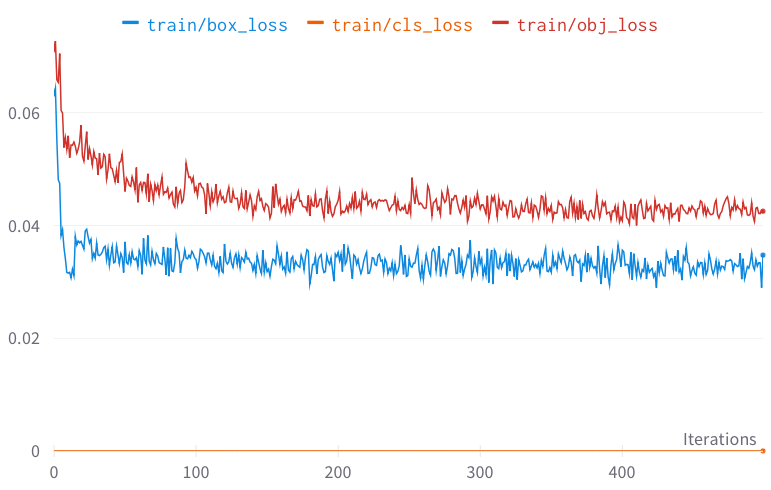
\includegraphics[width=0.8\linewidth]{./img/results/train.png}} \\
  \subfloat[Validação]{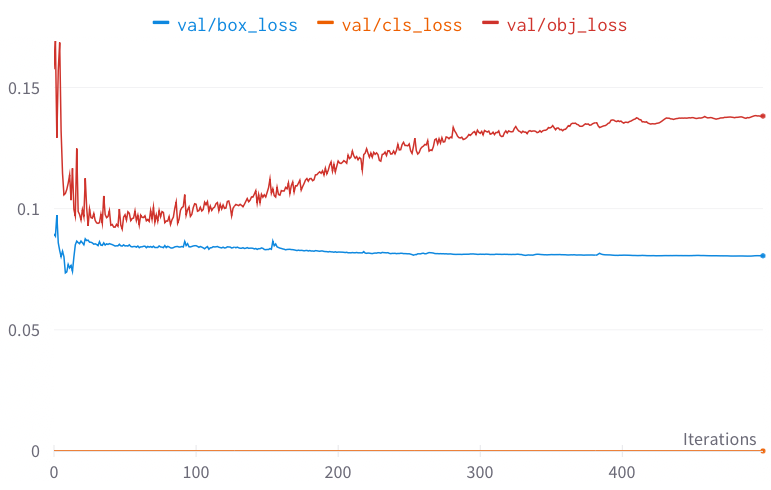
\includegraphics[width=0.8\linewidth]{./img/results/validation.png}}
 		\caption{Gráficos de monitoramento de métricas da YOLOv7 \emph{X} perante os conjuntos de treino e de validação.}  \label{fig:graph-train-val}
\end{figure}

 \begin{figure}[h!]
  	\centering
   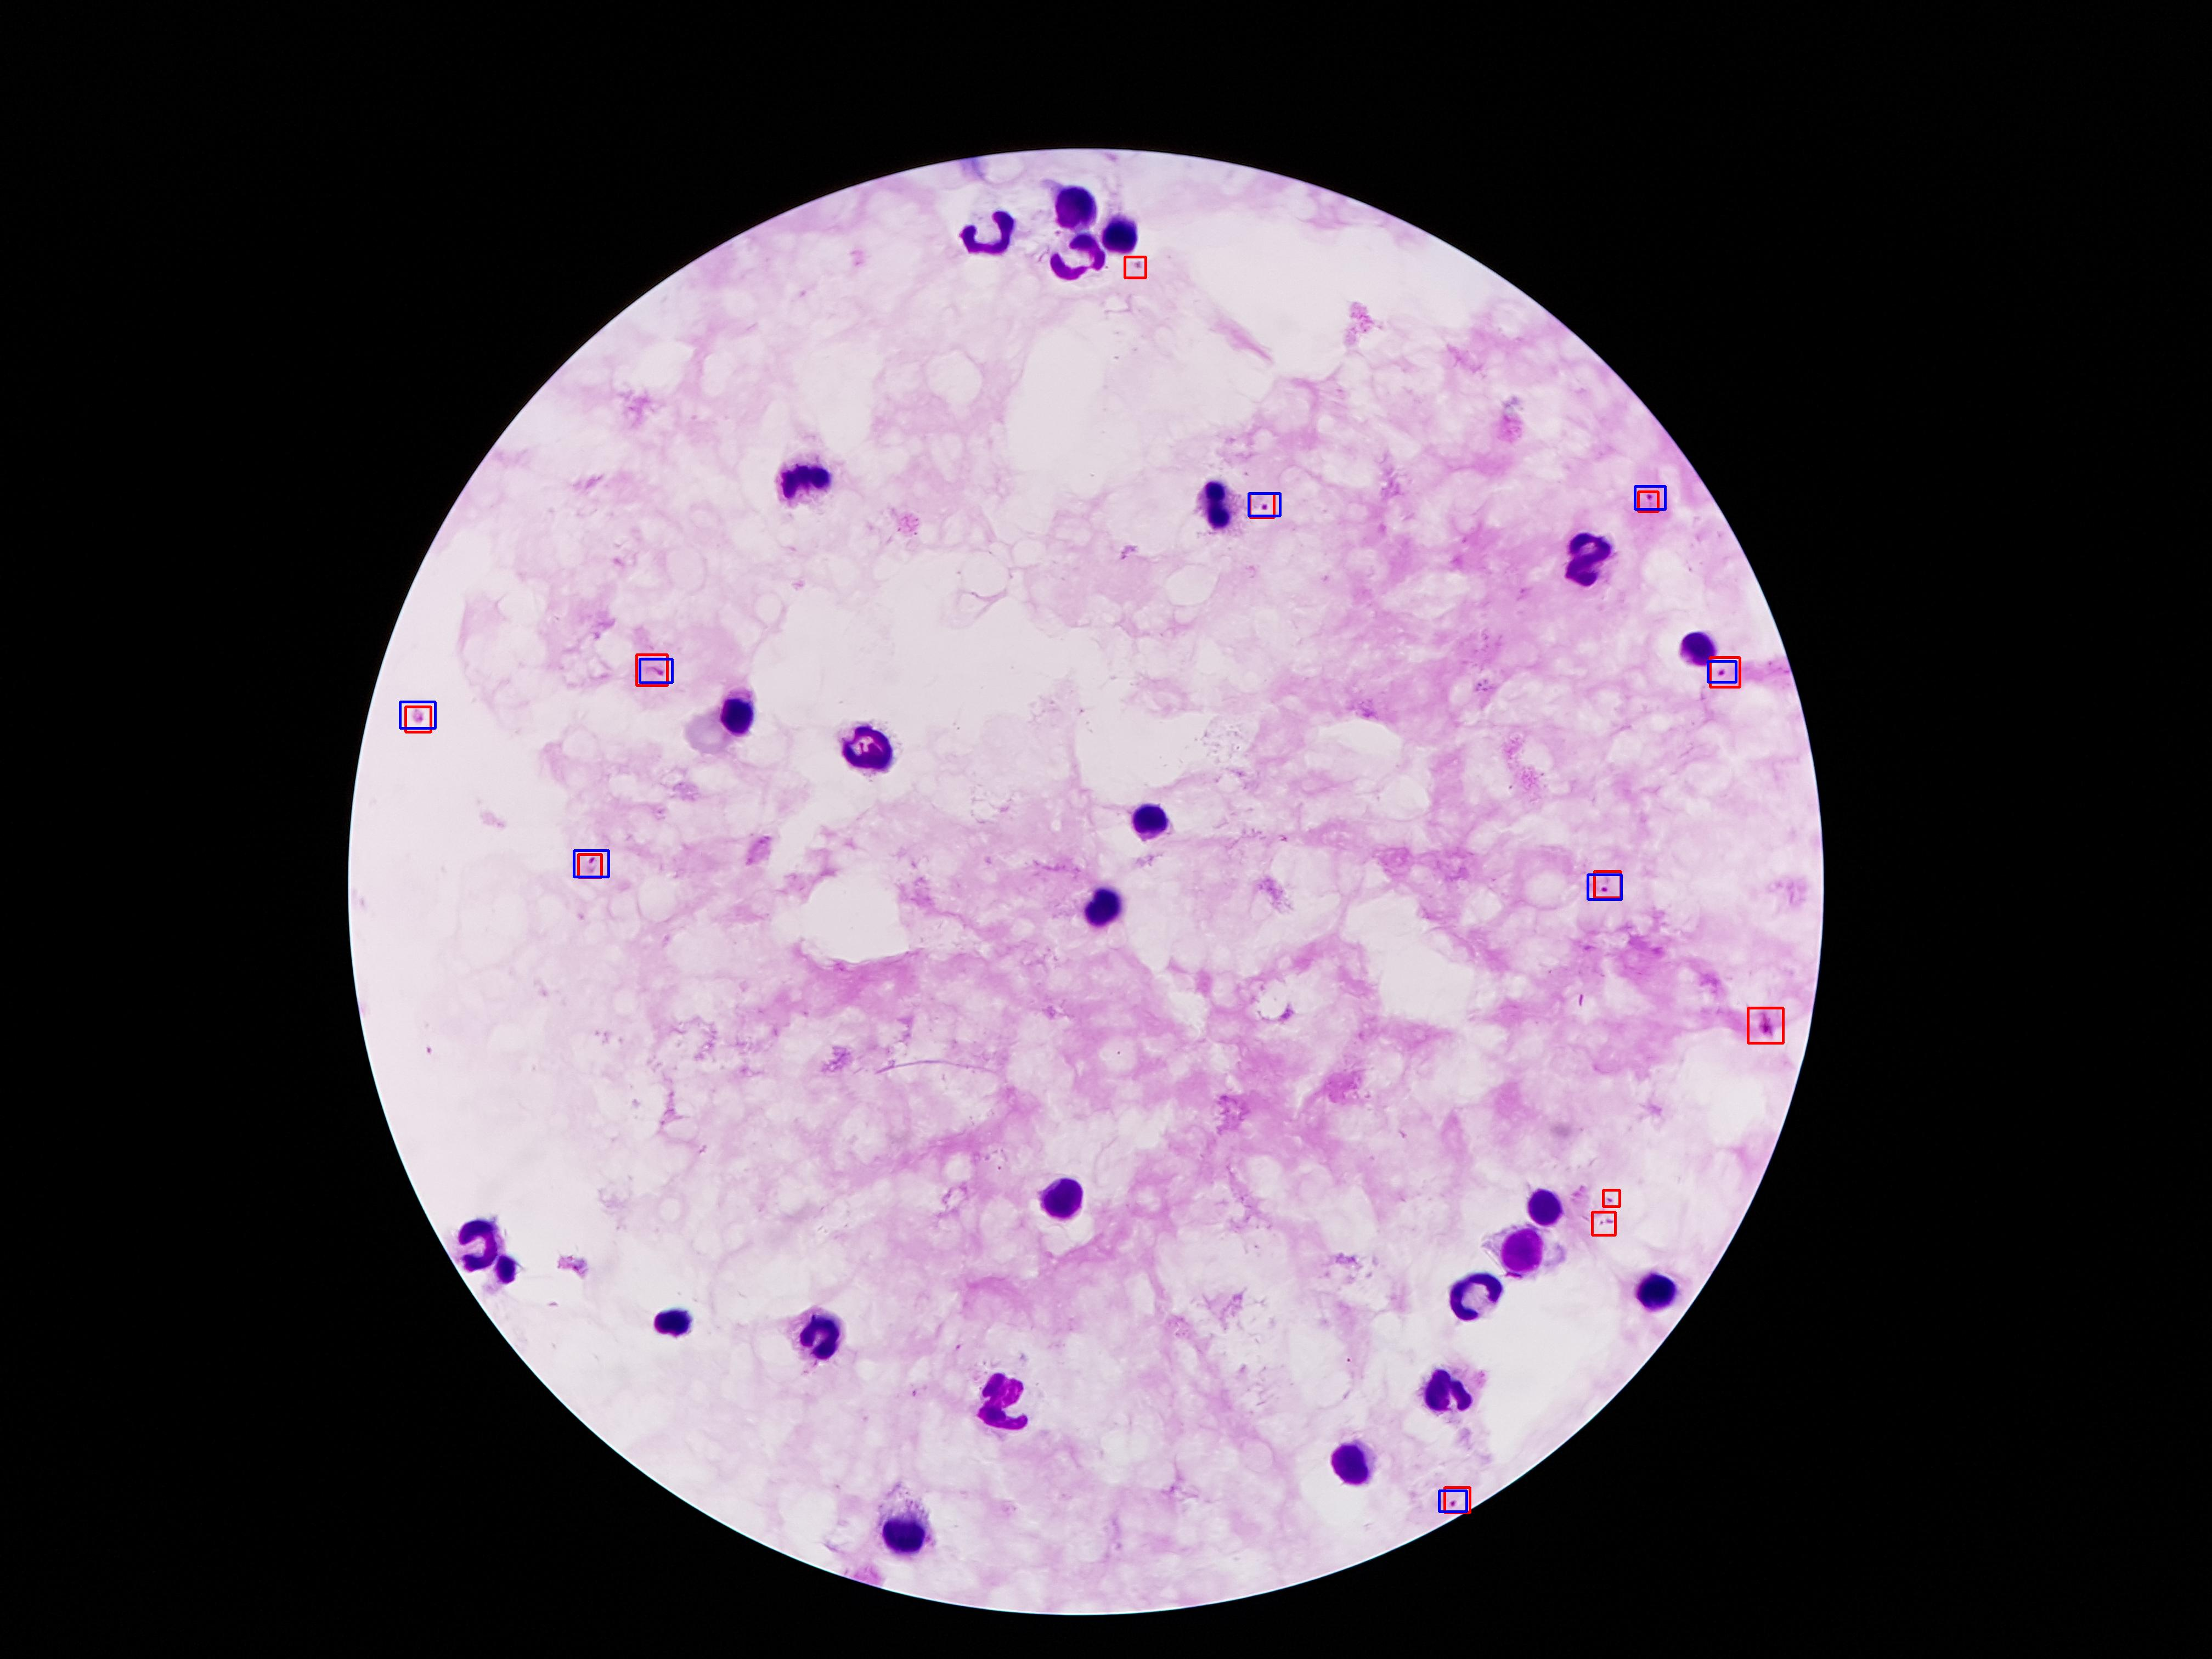
\includegraphics[width=\linewidth]{./img/full-predictions/result1-v7.jpg}
   \caption{Exemplo com poucos protozoários e suas respectivas detecções pela YOLOv7 \emph{X}.} \label{ex:poucos}
 \end{figure}

 \begin{figure}[h!]
  	\centering
   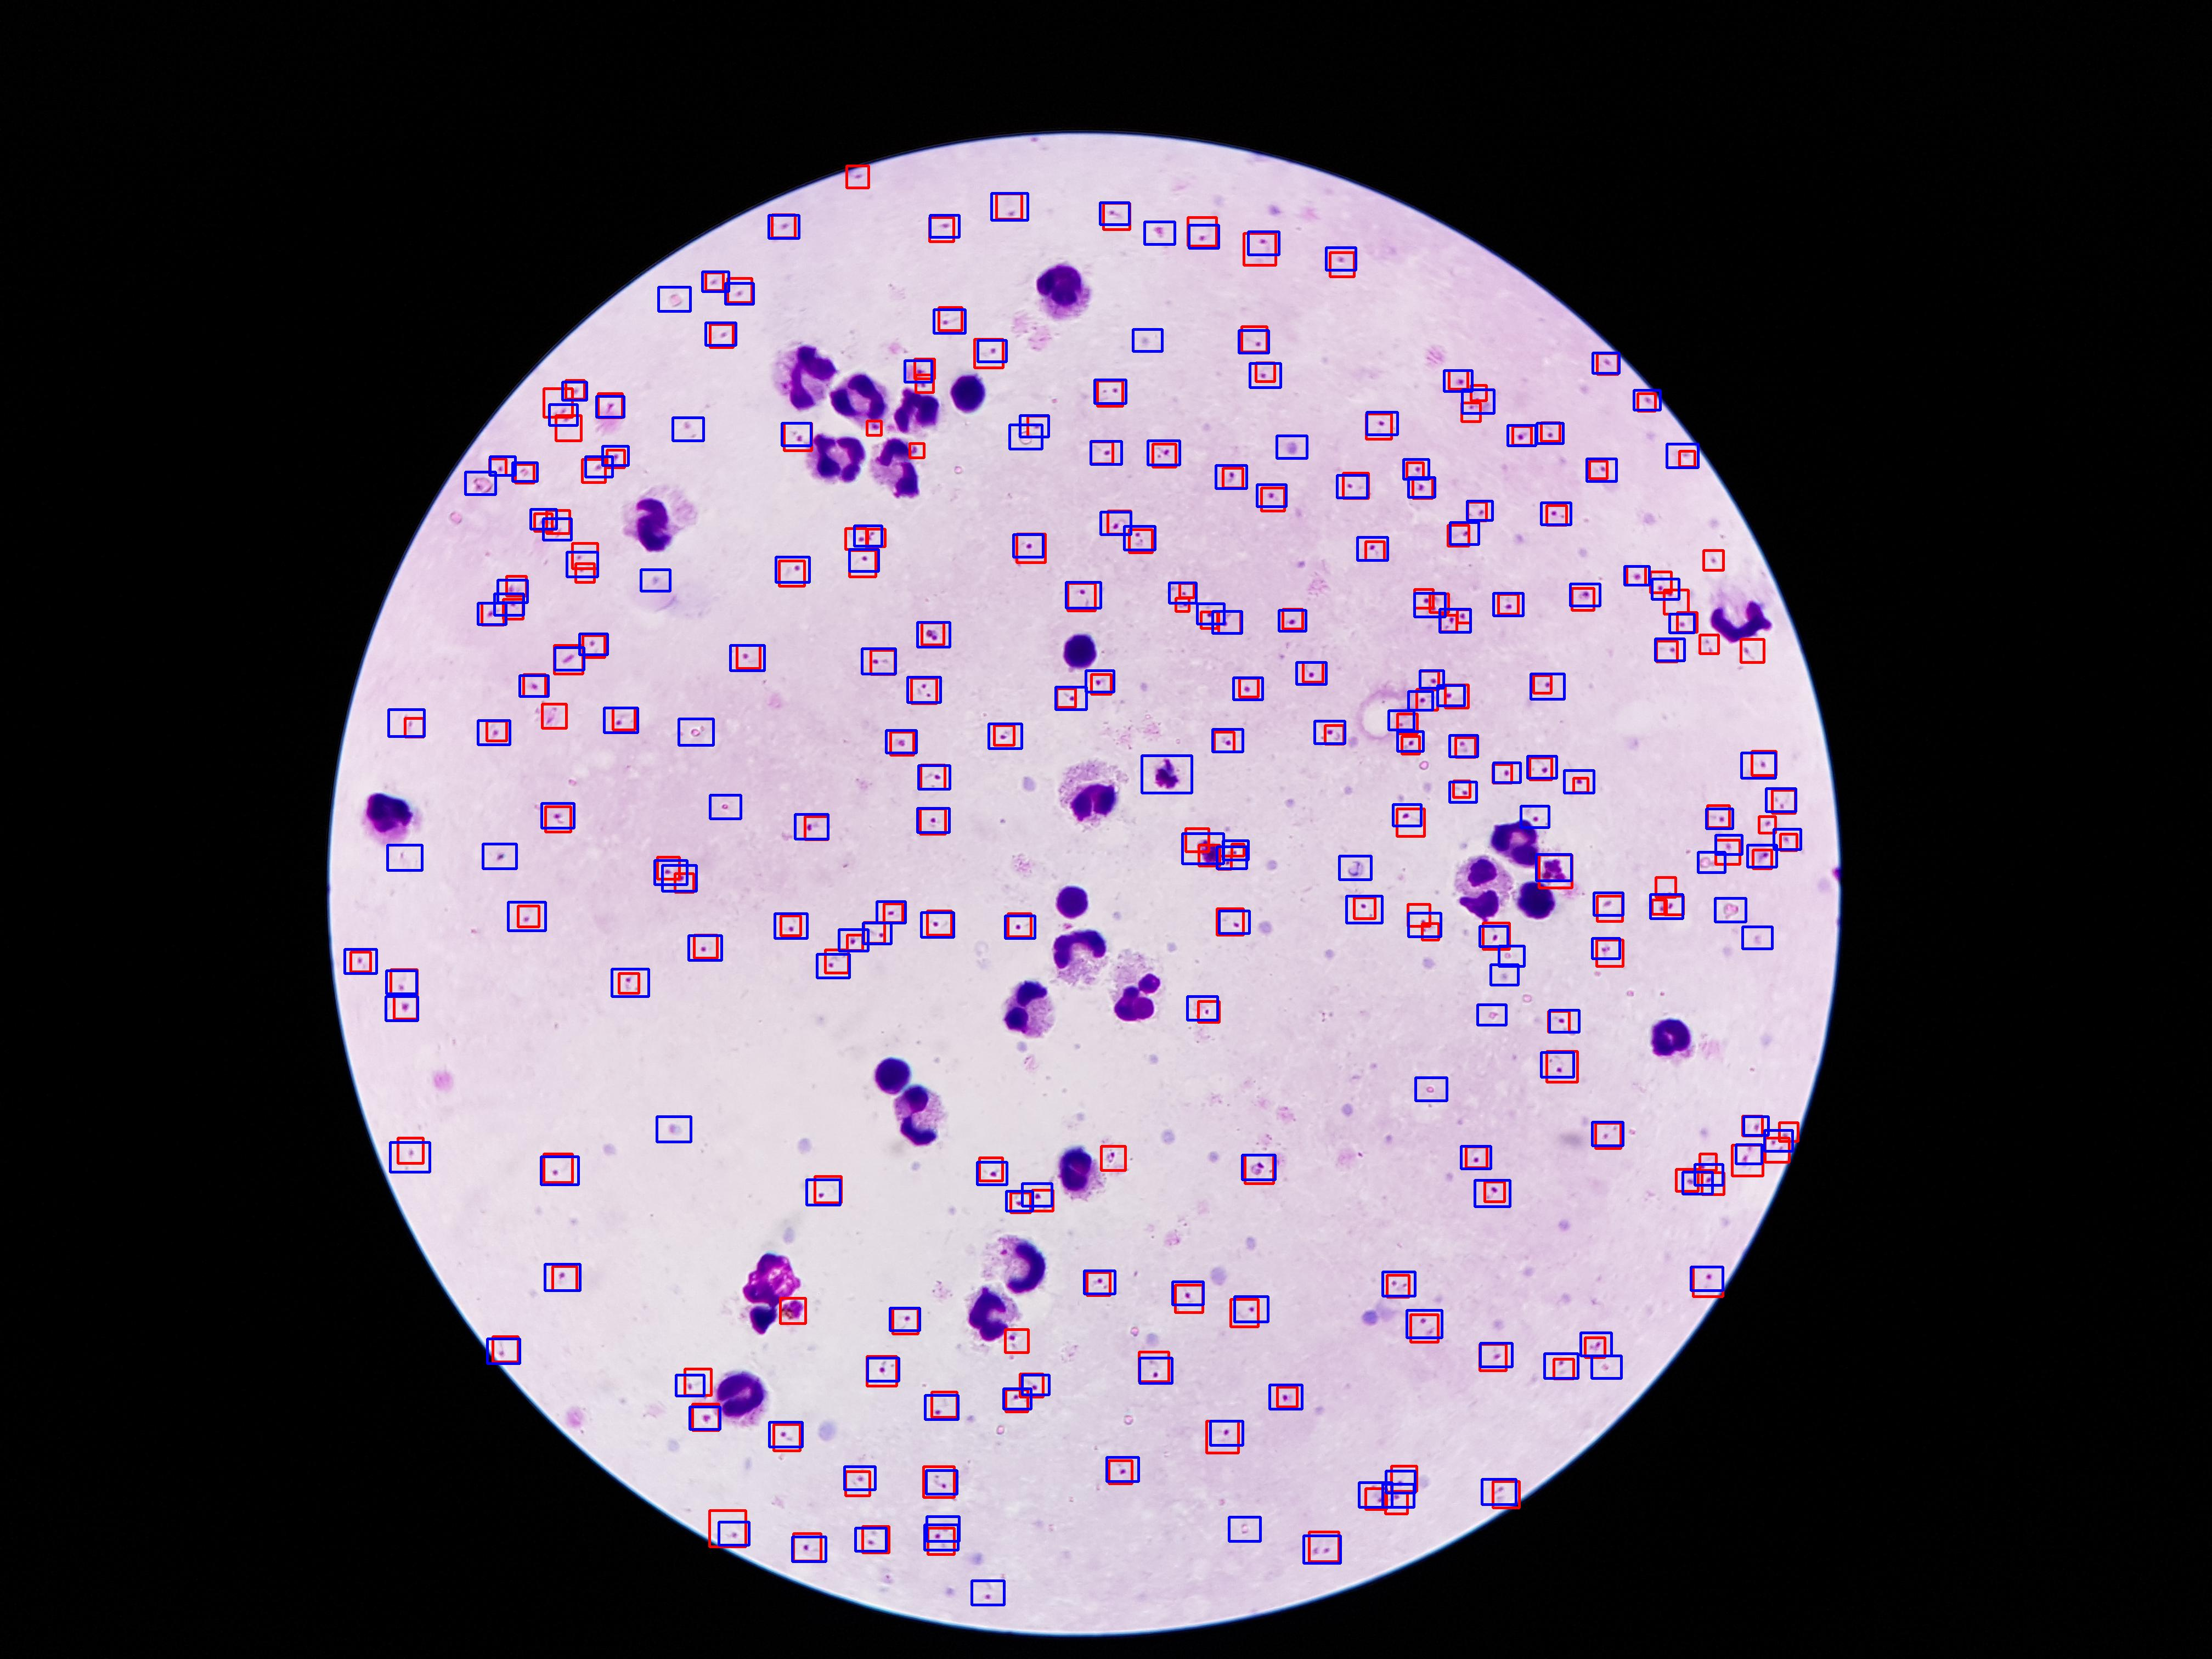
\includegraphics[width=\linewidth]{./img/full-predictions/result5-v7.jpg}
   \caption{Exemplo com muitos protozoários e suas respectivas detecções pela YOLOv7 \emph{X}.} \label{ex:muitos}
 \end{figure}

Apesar dos resultados superiores da YOLOv7 \emph{X} no tocante ao mAP@0.5 se mostrarem melhores que todos os demais modelos avaliados, não é possível afirmar a supremacia dessa solução perante as demais, haja vista, por exemplo, a menor precisão desse modelo frente à YOLOv5 \emph{Small}, a qual possui $\SI{90.09}{\percent}$ menos parâmetros. Seriam necessários mais experimentos e uma análise estatística cuidadosa para derivar conclusões nesse sentido. De maneira geral, todos os modelos mostraram-se competitivos para a tarefa, de natureza realística e com um grau de dificuldade acentuado pela área das caixas delimitadoras e pela distribuição uniforme de sua disposição nas imagens.




%!TEX root=../sbc-template.tex

\chapter{Considerações Finais e Trabalhos Futuros} \label{cap:considera}

O presente trabalho de conclusão de curso mostrou a viabilidade dos modelos de detecção de objetos baseados em \emph{Deep Learning} da Família YOLO no tocante à tarefa de detecção de protozoários causadoras de malária em imagens de lâminas de sangue oriundas de microscópio. Esses resultados foram observados a partir de experimentos computacionais com modelos YOLOv5 e YOLOv7 em uma base de dados realística da literatura contendo objetos pequenos e uniformemente distribuídos na imagem, o que a tornou especialmente desafiadora. As entradas dos modelos não necessitaram de pré-processamento computacional ou de intervenção humana para sua preparação para os modelos, o que se mostrou um avanço no estado da arte frente à outras contribuições identificadas na literatura. Os resultados evidenciaram a YOLOv7 \emph{X} como tendo melhor desempenho nos experimentos realizados, mas não foi possível assegurar a superioridade desse modelo frente aos demais, sendo necessários mais experimentos e também a ponderação quanto aos recursos computacionais disponível no âmbito de utilização da solução. Nesse sentido, ressalta-se que os resultados obtidos não se propõem em hipótese alguma a substituir especialistas humanos na tarefa, sendo essencial aprofundar as análises para verificar tal viabilidade.

Em trabalhos futuros almeja-se avaliar outras versões de modelos da Família YOLO recém propostos na literatura, tais como a YOLOv8 \cite{Jocher:YOLOv8}. Além disso, é importante validar o desempenho dos modelos em mais exemplos oriundos de mais localidades, especialmente da Região Amazônica onde tal doença é endêmica. Para tanto, encoraja-se pesquisadores de outras áreas a contribuir com bases de dados para esta tarefa de Visão Computacional.



% Referência segundo o padrão ABNT
% Edite este arquivo e inclua suas referências segundo a notação do Bibtex
\bibliography{ref}

\end{document}
